\documentclass[10pt,a4paper,spanish]{report}

\usepackage[spanish]{babel}
\usepackage[utf8]{inputenc}
\usepackage{amsmath, amsthm}
\usepackage{amsfonts, amssymb, latexsym}
\usepackage{enumerate}
\usepackage[official]{eurosym}
\usepackage{graphicx}
\usepackage[usenames, dvipsnames]{color}
\usepackage{colortbl}
\usepackage{multirow}
\usepackage{fancyhdr}
\usepackage[all]{xy}

% a4large.sty -- fill an A4 (210mm x 297mm) page
% Note: 1 inch = 25.4 mm = 72.27 pt
%       1 pt = 3.5 mm (approx)

% vertical page layout -- one inch margin top and bottom
\topmargin      0 mm    % top margin less 1 inch
\headheight     0 mm    % height of box containing the head
\headsep        10 mm    % space between the head and the body of the page
\textheight     250 mm
\footskip       14 mm    % distance from bottom of body to bottom of foot

\usepackage[bookmarks=true,
            bookmarksnumbered=false, % true means bookmarks in 
                                     % left window are numbered                         
            bookmarksopen=false,     % true means only level 1
                                     % are displayed.
            colorlinks=true,
            linkcolor=webblue]{hyperref}
\definecolor{webgreen}{rgb}{0, 0.5, 0} % less intense green
\definecolor{webblue}{rgb}{0, 0, 0.5}  % less intense blue
\definecolor{webred}{rgb}{0.5, 0, 0}   % less intense red

\newcommand{\HRule}{\rule{\linewidth}{0.5mm}} % regla horizontal para  el titulo

\pagestyle{fancy}
%con esto nos aseguramos de que las cabeceras de capítulo y de sección vayan en minúsculas

\renewcommand{\chaptermark}[1]{%
      \markboth{#1}{}}
\renewcommand{\sectionmark}[1]{%
      \markright{\thesection\ #1}}
\fancyhf{} %borra cabecera y pie actuales
\fancyhead[LE,RO]{\textcolor[rgb]{0.5,0.8,0.9}{\bfseries\thepage}}
\fancyhead[LO]{\bfseries\leftmark}
\renewcommand{\headrulewidth}{0.5pt}
\renewcommand{\footrulewidth}{0pt}
\addtolength{\headheight}{0.5pt} %espacio para la raya
\fancypagestyle{plain}{%
      \fancyhead{} %elimina cabeceras en páginas "plain"
      \renewcommand{\headrulewidth}{0pt} %así como la raya
}

%%%%% Para cambiar el tipo de letra en el título de la sección %%%%%%%%%%%
\usepackage{sectsty}
\chapterfont{\fontfamily{pag}\selectfont} %% for chapter if you want
\sectionfont{\fontfamily{pag}\selectfont}
\subsectionfont{\fontfamily{pag}\selectfont}
\subsubsectionfont{\fontfamily{pag}\selectfont}


%Definimos autor y título
\title{Ingeniería, empresa y sociedad: \\ Parcial 2}
\author{Marta Gómez Macías}

\begin{document}
      \begin{titlepage}
            \begin{center}
                  \HRule \\[0.4cm]
                  \textsc{\LARGE \textcolor[rgb]{0.2,0.8,0.4}Ingeniería, \textcolor[rgb]{0.5,0.1,0.5}Empresa y \textcolor[rgb]{0.7,0.8,0.9}Sociedad:}\\[1.5cm]
                  \textsc{\Large \textbf{P}arcial 2}\\[0.5cm]
                  \HRule \\[1.5cm]
                  \begin{flushleft}
                        \emph{Hecho por:}\\
                        Marta \textsc{Gómez Macías}
                  \end{flushleft}
                  \vspace{10cm}
                  {\Large \today}
                  \vspace{5mm}
                  \\
                  \htmladdnormallink{
\includegraphics[width=2cm]{88x31.png}}
            {http://creativecommons.org/licenses/by-nc/4.0/}\\
            \texttt{Ingeniería, Empresa y Sociedad: Parcial 2 by 
            \href{mailto:mgmacias95@gmail.com}{Marta Gómez Macías}
            is licensed under a \htmladdnormallink{Creative Commons
            Reconocimiento-NoComercial-CompartirIgual 4.0 Internacional License}
            {http://creativecommons.org/licenses/by-nc/4.0/}}.
            \end{center}
      \end{titlepage}

      \setcounter{chapter}{4}

      \tableofcontents

\chapter{\textcolor[rgb]{0.3,0.4,0.6}{El Entorno de la empresa}}
      \section{\textcolor[rgb]{0.3,0.4,0.6}Definición del entorno}
            Desde que las organizaciones se consideraron como sistemas abiertos, el entorno pasó a tener un papel relevante para su estudio. El entorno engloba todo aquello \textit{\textcolor[rgb]{0.3,0.4,0.6}{ajeno}} a la empresa como organización. Se trata de un concepto que incluye la totalidad de fuerzas externas que pueden influir en algún aspecto de la actividad organizacional o sobre sus resultados. El entorno está formado por todos los factores que pueden incidir, en el presente o en el futuro, en sus actuaciones y/o resultados, los \textit{\textcolor[rgb]{0.3,0.4,0.6}{factores estratégicos}}:

            \[\xygraph{
            [] *+[F]+[o]{\text{Factores Estratégicos}}
            :[ddll] *+=[o]=<30mm>[F=]{Oportunidades}
            ,:[ddrr] *+=[o]=<30mm>[F=]{Amenazas}
            }\]

            Entre la organización y su entorno existen unos límites que determinan el grado de apertura de ésta como sistema y su permeabilidad frente a los factores del entorno. La función principal de los límites es actuar como filtros. Gracias a los límites, las empresas también pueden actuar con independencia y autonomía frente a la intrusión de fuerzas del entorno.

            Tales límites, son difíciles de establecer, pues las organizaciones son instituciones sociales integradas por personas cuyo comportamiento se rige por factores sociológicos y psicológicos. Starbuck comparó el problema de encontrar los límites de la organización con el de encontrar los límites de una nube.

            Miles, Snow y Pfeffer consideran que aplicar esta idea a las organizaciones supone definir los límites en función de los modelos de interacción y del grado de implicación entre diferentes individuos y grupos. Sin embargo, como las organizaciones son sistemas abiertos, el principal inconveniente es que la densidad de las interacciones está en constante cambio, y por tanto, los límites se van alterando.
            \newpage
            Por otro lado, la delimitación del entorno también implica definir un ámbito de referencia o alcance del medio en el que la empresa opera o puede hacerlo. Según Bueno, pueden establecerse varios \textit{\textcolor[rgb]{0.3,0.4,0.6}{niveles del entorno}}: 
            \begin{enumerate}
                  \item Global.
                  \item Internacional (multipaís).
                  \item Doméstico (país).
                  \item Regional.
                  \item Local (nicho).
            \end{enumerate}

            El nivel en el que una empresa define su entorno influye en las actividades que realiza y en cómo interactúa con las fuerzas que se derivan de éste. La mayoría de las empresas se enfrentan a entornos globales, compitiendo con empresas de todo el mundo, y desplegando sus actividades más allá de las fronteras del propio país.

            \begin{figure}
                  \centering
                  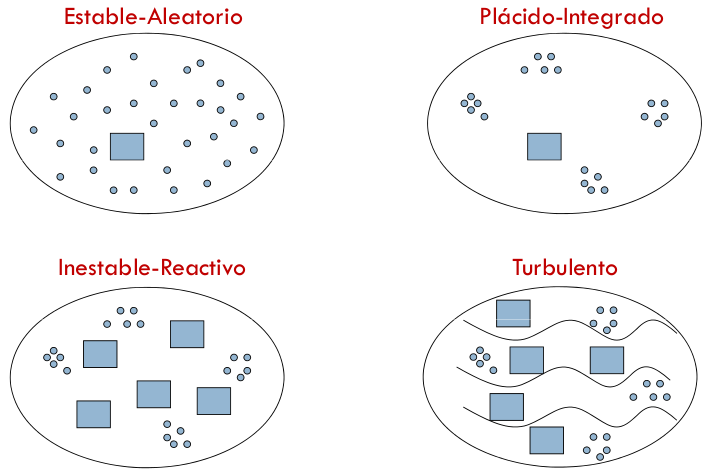
\includegraphics[width=0.8\textwidth]{1}
                  \caption{Tipos de entorno}
                  \label{tipos_entorno}
            \end{figure}

    \section{\textcolor[rgb]{0.3,0.4,0.6}Características del entorno}

        Para conocer cómo interactúa el entorno con la empresa es necesario identificar las características o atributos que definen unos entornos frente a otros. Las características del entorno son los atributos del entorno a los que se enfrenta una organización. Estas características se han estudiado desde dos perspectivas, en función de la consideración del entorno como una fuente de recursos o una fuente de incertidumbre.

        Desde la primera perspectiva, se considera que el entorno es un conjunto de recursos humanos, materiales y de información. Como ninguna organización es capaz de generar todos los recursos que necesita, ni de realizar todas las actividades que le permitan sobrevivir por sí misma, la empresa requiere conocer si el entorno posee un elevado número de recursos, si son variados, si están concentrados, si existen otras empresas que compiten por ellos, etc. En base a la combinación de las características mencionadas existirán cuatro tipos de entornos: estable-aleatorio, plácido-integrado, inestable-reactivo y turbulento (Véase \hyperref[tipos_entorno]{Figura \ref*{tipos_entorno}}):
            \begin{description}
                  \item[Entorno estable-aleatorio]: la empresa no compite con otras por los recursos, además, los recursos están dispersos, es decir, distribuidos aleatoriamente (de fácil acceso) y son abundantes.
                  \item[Entorno plácido-integrado]: los recursos permanecen estables, pero tienden a agruparse; la concentración de recursos tiene importancia porque algunas posiciones en el entorno son más ricas o ventajosas que otras.
                  \item[Entorno inestable-reactivo]: los cambios son relativamente pocos, pero está presente más de una empresa con similares necesidades de recursos. Los movimientos de una empresa dentro del entorno probablemente irán acompañados de movimientos de otras empresas similares.
                  \item[Entorno turbulento]: no sólo existe competencia entre empresas, sino que las condiciones generales y recursos disponibles que afectan a todas están en continuo cambio.
            \end{description}

            Desde la perspectiva del entorno como fuente de incertidumbre, se considera que el entorno es una fuente de información para tomar decisiones sobre la estructura o las actividades que realizan las organizaciones. La principal preocupación respecto al entorno es la incertidumbre que éste puede generar en la información que es percibida por las personas que toman decisiones. 

            Un entorno es \textit{\textcolor[rgb]{0.3,0.4,0.6}{incierto}} cuando no hay información o la misma es difícil de predecir en relación a:
            \begin{enumerate}[1.]
                  \item los factores del entorno que afectan a una situación dada.
                  \item Cuáles serán las reacciones de los factores del entorno ante una determinada decisión de la empresa.
                  \item Cómo afectan los factores del entorno al resultado de la empresa.
            \end{enumerate}

            Los dos enfoques del entorno que se han expuesto no son excluyentes, pues las características del entorno que se derivan de ambos están relacionadas.

            Podemos aproximar las dos perspectivas y establecer las características del entorno basándonos en cuatro dimensiones:

            \[\begin{xy}
            ,(0,0)*+=<20mm>[F]\txt<3cm>{{\small Dinámico} {\tiny (Variaciones de los factores del entorno, numerosas, profundas, rápidas e impredecibles)}}
            \ar@{<->}
            ,(60,0)*+=<20mm>[F]\txt<3cm>{{\small Estable} {\tiny (Sin cambios o cambios predecibles)}}
            \end{xy}\]
            \[\begin{xy}
            ,(0,0)*+=<20mm>[F]\txt<3cm>{{\small Complejo} {\tiny (Grandes conocimientos sofisticados sobre productos, clientes o factores)}}
            \ar@{<->}
            ,(60,0)*+=<20mm>[F]\txt<3cm>{{\small Sencillo} {\tiny (El conocimiento se puede racionalizar o hacerse más comprensible)}}
            \end{xy}\]
            \[\begin{xy}
            ,(0,0)*+=<20mm>[F]\txt<3cm>{{\small Diverso} {\tiny (Gran número de clientes, productos, servicios o zonas geográficas que abastecer)}}
            \ar@{<->}
            ,(60,0)*+=<20mm>[F]\txt<3cm>{{\small Integrado} {\tiny (Variables reducidas y similares)}}
            \end{xy}\]
            \[\begin{xy}
            ,(0,0)*+=<20mm>[F]\txt<3cm>{{\small Hostil} {\tiny (Mayor competencia y disponibilidad de recursos)}}
            \ar@{<->}
            ,(60,0)*+=<20mm>[F]\txt<3cm>{{\small Munificiente} {\tiny (Menor competencia y disponibilidad de recursos)}}
            \end{xy}\]
            \[\begin{xy}
            ,(0,0)*+=<20mm>[]\txt{{\small Mayor incertidumbre}}
            \ar@{<->}
            ,(60,0)*+=<20mm>[]\txt{{\small Menor incertidumbre}}
            \end{xy}\]

            \begin{description}
                  \item[Estabilidad-Dinamismo]: Un entorno dinámico no sólo indica que existen cambios, sino que éstos son impredecibles. Un entorno es estable cuando no se producen cambios en los factores que influyen a la empresa o se pueden predecir con facilidad.
                  \item[Simplicidad-Complejidad]: Un entorno es complejo en la medida en que requiere que la organización disponga de gran cantidad de conocimientos sofisticados sobre los productos, clientes o factores. Sin embargo, se puede volver sencillo cuando dicho conocimiento puede racionalizarse o se hace más comprensible.
                  \item[Integración-Diversificación]: Un entorno es diverso por la existencia de un gran número de clientes, de productos, servicios o zonas geográficas que abastecer. Un entorno es integrado si las variables que lo constituyen son reducidas y similares.
                  \item[Munificación-Hostilidad]: La hostilidad está influida por la competencia, por las relaciones de la organización con los sindicatos, gobiernos y otros grupos externos, así como por la disponibilidad de los recursos a los que puede acceder. A menor competencia y mayor disponibilidad de recursos, el entorno es más munificiente.
            \end{description}

            Estas características poseen una relación positiva con la incertidumbre. El entorno es más incierto cuanto más dinámico, complejo, diverso y hostil sea. La mayoría de las empresas operan en entornos con características que tienden a aumentar la incertidumbre.

    \section{\textcolor[rgb]{0.3,0.4,0.6}Análisis del entorno general}

        Para abordar qué factores del entorno son relevantes para la organización, se acepta la distinción entre \textit{\textcolor[rgb]{0.3,0.4,0.6}{entorno general}} y \textit{\textcolor[rgb]{0.3,0.4,0.6}{entorno específico}}.

        El \textbf{entorno general} está integrado por un conjunto de factores, que pueden ejercer influencia sobre todas las empresas dentro de un determinado sistema socioeconómico. El entorno genérico agrupa a todos los elementos que pueden afectar de forma similar al conjunto de las organizaciones en un tiempo y espacio dados. Estos factores pueden simplificarse en cuatro categorías:
            \begin{description}
                  \item[Económicos]: Factores relativos al marco económico general.
                  \item[Socioculturales]: Factores vinculados a los antecedentes históricos, ideologías, valores y normas de la sociedad, el nivel educativo, la igualdad social, etc.
                  \item[Políticos-Legales]: Factores relacionados con el sistema político y su estabilidad, así como todo tipo de leyes civiles, comerciales, laborales, fiscales\ldots, que constituyen elementos normativos para las empresas.
                  \item[Tecnológicos]: Nivel científico y tecnológico de la sociedad que determina el grado en el que la comunidad científica y tecnológica es capaz de desarrollar nuevos conocimientos y aplicarlos (porcentaje del PIB destinado a investigación, número de investigadores, etc.)
            \end{description}

            En las últimas dos décadas se han constatado grandes cambios en cada una de estas dimensiones de los factores del entorno general, debido a la existencia de un gran dinamismo y complejidad. Los efectos que tales cambios pueden producir en las empresas son considerados como oportunidades y amenazas. Las \textit{\textcolor[rgb]{0.3,0.4,0.6}{oportunidades}} son efectos positivos que deben ser aprovechados para crecer o mejorar los resultados de la organización. Las \textit{\textcolor[rgb]{0.3,0.4,0.6}{amenazas}} representan los impactos negativos sobre la empresa. Un buen directivo debe convertir las amenazas en oportunidades, y estar alerta a las nuevas oportunidades que puedan derivarse.

            El estudio de los efectos de los cuatro factores del entorno general expuestos se conoce por el acrónimo de \textit{\textcolor[rgb]{0.3,0.4,0.6}{análisis PEST (Político-legal, Económico, Sociocultural, Tecnológico)}}. Este análisis permite elaborar una lista de factores principales en cada categoría y evaluar para cada uno de ellos sus efectos como amenaza o como oportunidad.
            Las etapas en un análisis PEST son:
            \begin{enumerate}[1.]
                  \item Delimitación de los factores estratégicos del entorno.
                  \item Descripción de la evolución de los factores estratégicos del entorno.
                  \item Valorización y jerarquización de oportunidades y amenazas
            \end{enumerate}
            Y las consideraciones que debemos tener en cuenta al hacer un análisis PEST son:
            \begin{enumerate}
                  \item No todos los factores son estratégicos. Algunos factores sólo afectan a determinadas empresas, a pesar de ser analizados en el entorno general
                  \item Los factores pueden ser fuente de oportunidades y de amenazas a la vez para distintos actores.
                  \item La finalidad de un análisis PEST no es describir a un país desde el punto de vista económico, social, político o tecnológico, sino que su objetivo es conocer las oportunidades y amenazas que el contexto puede significar para la supervivencia de una empresa concreta.
            \end{enumerate}

            Para completar el análisis del entorno general en el caso de \underline{empresas globales}, se podría utilizar el ``\textbf{Diamante de Porter}'' para observar las influencias del entorno en el contexto de la competencia global. Según Porter, hay una serie de razones inherentes a cada país para explicar que unos sean más competitivos que otros y que algunos sectores dentro de cada país sean más competitivos que otros. Así podemos destacar:
            \begin{enumerate}
                  \item Las condiciones de factores específicos que permiten explicar la base de la ventaja a escala nacional (recursos naturales o el clima).
                  \item Las condiciones de la demanda nacional que constituyen la base de las características de las ventajas de una organización.
                  \item El que una industria de éxito pueda crear ventajas competitivas para otras industrias relacionadas y de soporte.
                  \item El contexto de las características de la estrategia de la empresa, la estructura y la rivalidad en diferentes países.
            \end{enumerate}
            \begin{center}
            {\LARGE \textcolor[rgb]{0.3,0.4,0.6}{Teoría de la competitividad de las ubicaciones}}
            % \framebox[1.1\width]{\txt{\textbf{Estatregia y estructura}:\\ en cada país se produce\\ un tipo de estructuras\\ y liderazgos que es más \\apropiado para \\algunas actividades}}
            \[\begin{xy}
            ,(0,0)*+=[o]=<3cm>[F]\txt<3cm>{Contexto de la estrategia de empresa, estructura y rivalidad en\\países}
            ,(0,60)*+=[o]=<3cm>[F]\txt<3cm>{Industrias de éxito\\{\tiny Industrias de soporte e industrias relacionadas}}
            ,(-60,30)*+=[o]=<3cm>[F]\txt<3cm>{Condiciones de los factores productivos específicos\\{\tiny Ventaja nacional}}
            ,(60,30)*+=[o]=<3cm>[F]\txt<3cm>{Condiciones de demanda nacional\\{\tiny Ventaja organizacional}}
            \ar@{<->} (0,15);(0,45)
            \ar@{<->} (-45,30);(45,30)
            \ar@{<->} (0,45);(45,30)
            \ar@{<->} (45,30);(0,15)
            \ar@{<->} (0,15);(-45,30)
            \ar@{<->} (-45,30);(0,45)
            \end{xy}\]
            % \framebox[1.1\width]{\txt{\textbf{Rivalidad}:\\Cuanto mayor sea la\\rivalidad interna,\\mayor la presión para\\innovar y reducir costes}}
            \end{center}

      \section{\textcolor[rgb]{0.3,0.4,0.6}Análisis del entorno específico}

            El \textbf{entorno específico} es el ambiente más próximo de cada organización, por tanto, ejerce una influencia directa en la misma. También se denomina \textit{\textcolor[rgb]{0.3,0.4,0.6}{entorno operativo}}, por estar compuesto por las fuerzas más específicas e importantes de los procesos de transformación y toma de decisiones de la organización. Los factores de este entorno son ``potencialmente relevantes para el establecimiento y el logro de los objetivos de la organización''.

            Los componentes del entorno específico son:
            \begin{enumerate}
                  \item Proveedores de \textit{\textcolor[rgb]{0.3,0.4,0.6}{inputs}}.
                  \item Clientes.
                  \item Competidores.
                  \item Entidades reguladoras.
            \end{enumerate}

            El entorno específico puede ser analizado desde una perspectiva industrial mediante el análisis de las fuerzas competitivas que operan en un determinado sector y que componen el entorno competitivo. Porter propone un modelo de estudio que se conoce como el de \textit{\textcolor[rgb]{0.3,0.4,0.6}{rivalidad ampliada}} o de \textit{\textcolor[rgb]{0.3,0.4,0.6}{las cinco fuerzas}}. Estas cinco fuerzas determinan la rentabilidad de una empresa en un determinado sector industrial:
            \begin{enumerate}
                  \item Competidores actuales
                  \item Competidores potenciales
                  \item Productos sustitutos
                  \item Poder de negociación
                  \item Poder de negociación de los proveedores
            \end{enumerate}
            \[\begin{xy}
            ,(0,0)*+=[F=]=<6cm>\txt<3cm>{Competidores del sector \\ \\ \\ Rivalidad entre empresas\\existentes}
            ,(0,-40)*+=[F]=<3cm>\txt{Sustitutos}
            ,(-25,-40)*+=[]=<3cm>\txt{Amenaza de los\\productos sustitutos}
            ,(0,40)*+=[F]=<3cm>\txt{Competidores\\potenciales}
            ,(30,40)*+=[]=<3cm>\txt{Amenaza de los\\nuevos competidores}
            ,(60,0)*+=[F]=<3cm>\txt{Clientes}
            ,(60,10)*+=[]=<3cm>\txt{Poder de negociación\\de clientes}
            ,(-60,0)*+=[F]=<3cm>\txt{Proveedores}
            ,(-60,-15)*+=[]=<3cm>\txt{Poder de negociación\\de proveedores}
            ,(-60,40)*+=[]=<3cm>\txt{Entorno\\competitivo}
            \ar@{=>} (0,-32);(0,-15)
            \ar@{=>} (53,0);(15,0)
            \ar@{=>} (-50,0);(-15,0)
            \ar@{=>} (0,29);(0,15)
            \end{xy}\]
            \newpage
            Los \textit{\textcolor[rgb]{0.3,0.4,0.6}{competidores actuales}}, son el conjunto de empresas que compiten por los clientes en un sector industrial, entendiendo sector industrial como el conjunto de empresas que desarrollan una misma actividad económica y venden productos bien definidos o líneas de productos afines.

            La intensidad de la competencia es el resultado de una serie de factores estructurales, tales como:
            \begin{description}
                  \item[Número de competidores y equilibro entre competidores]: Cuanto mayor es el número de competidores establecidos y el equilibrio entre los mismos, mayor será la intensidad de la competencia.
                  \item[Ritmo de crecimiento de la industria]: A medida que el ritmo de crecimiento de la industria se reduce, la intensidad de la competencia se incrementa.
                  \item[Barreras de movilidad]: Son aquellos obstáculos que impiden o dificultan a las empresas moverse de un segmento a otro dentro de la misma industria. Protegen a la empresa dentro del segmento, por lo que su intensidad para el conjunto de la industria decrece.
                  \item[Barreras de salida]: Son factores que impiden o dificultan el abandono de una industria por parte de una empresa. Las barreras de salida fuerzan a luchar para sobrevivir y seguir compitiendo en la industria, por lo que la intensidad de la competencia aumenta. Se pueden clasificar en:
                  \begin{enumerate}
                        \item Activos especializados.
                        \item Costes fijos de salida.
                        \item Barreras emocionales.
                        \item Interrelaciones estratégicas entre negocios.
                        \item Presiones sociales/gubernamentales.
                  \end{enumerate}
                  \item[Estructura de costes de las empresas]: un mayor volumen de los costes fijos (no varían con la producción) o variables (sí varían con la producción) hace que las empresas operen a plena capacidad para reducir sus costes medios, incrementando así la intensidad de la competencia. \\
                  \begin{center}
                        $\txt{Coste total}=\txt{Costes Variables}+\txt{Costes Fijos}$ \\
                        $\txt{Si producción=0} \rightarrow \txt{Coste total}=0+\txt{Costes Fijos}$
                  \end{center}
                  \item[Diferenciación de productos]: A medida que en una industria exista un mayor nivel de diferenciación de productos, la intensidad de la competencia se reduce, ya que los clientes fidelizan con los distintos productos diferenciados.
                  \item[Costes de cambio]: La existencia de costes de cambio de proveedores reduce la intensidad de la competencia, al vincularse más estrechamente unos y otros. Entendemos como costes de cambio los obstáculos que existen e impiden la finalización de la relación actual y el cambio a un proveedor alternativo.
                  \item[Capacidad productiva instalada]: Cuando por diferentes motivos las empresas de un sector aumentan su capacidad productiva, y en su conjunto la oferta del sector supera a la demanda, las empresas tenderán a ser más competitivas para evitar encontrarse con un exceso de capacidad y los costes derivados de dicha situación.
                  \item[Diversidad de competidores]: Cuando los competidores difieren en estrategias, personalidad, relaciones con sus compañías matrices\ldots pueden interferir continuamente unos sobre otros, provocando efectos intensificadores de la competencia.
                  \item[Intereses estratégicos]: A medida que más empresas estén interesadas simultáneamente en lograr el éxito en una industria, la competencia se intensifica, ya que estarán dispuestas a desarrollar diferentes acciones que les conduzcan a ese fin, aunque tengan que sacrificar momentáneamente sus resultados.
            \end{description}

            En segundo lugar, los \textit{\textcolor[rgb]{0.3,0.4,0.6}{competidores potenciales}} son empresas que pueden estar interesadas en entrar en el sector. Las posibilidades de que estos competidores potenciales puedan competir con los actuales dependen de las \textbf{barreras de entrada al sector} y de la \textbf{reacción de los competidores establecidos ante un nuevo ingreso}. Dicha reacción depende de:
            \begin{enumerate}
                  \item Tradición de represalias en la industria.
                  \item Empresas existentes (empresas del sector) que tengan fuertes recursos para defenderse.
            \end{enumerate}
            Estos factores desmotivarán la entrada de un nuevo competidor.

            Por \textit{\textcolor[rgb]{0.3,0.4,0.6}{barreras de entrada}} entendemos todos aquellos mecanismos que dificultan o impiden el ingreso de nuevas empresas al sector, normalmente mediante la disminución de las expectativas de rentabilidad de los posibles nuevos competidores. Las principales barreras de entrada son:
            \begin{description}
                  \item[Economías de escala y alcance]: las empresas que intenten entrar deben hacerlo a gran escala, pues si entran en pequeña escala deben soportar desventajas en costes.\footnote{Las economías de escala: a mayor producción menor precio, ya que obtenemos descuentos por volumen y el coste fijo se reparte entre un mayor número de unidades producidas.}
                  \item[Diferenciación de producto]: Obliga al que quiere entrar a realizar grandes inversiones para superar la fidelidad existente.
                  \item[Necesidades de capital]: Es necesario invertir grandes recursos financieros para competir.
                  \item[Costes de cambio a los que tiene que hacer frente el cliente al cambiar de proveedor]: Ante costes elevados, los proveedores de nuevo ingreso deben ofrecer una gran reducción de precios o una mejora en el rendimiento del producto para que el cliente cambie de proveedor.
                  \item[Acceso a los canales de distribución]: Si estos canales están dominados por las empresas actuales, las nuevas empresas deben convencer a los canales de que acepten sus productos cediendo algo y reduciendo sus beneficios.
                  \item[Desventajas en costes diferentes de las economías de escala]: Estos perjudican a los competidores potenciales.
                  \item[Política gubernamental]: El gobierno puede limitar o impedir la entrada a determinadas industrias.
            \end{description}

            En tercer lugar, los \textit{\textcolor[rgb]{0.3,0.4,0.6}{productos sustitutivos}} son los productos que desempeñan las mismas funciones desde el punto de vista de los clientes. Cuantos más productos sustitutivos existan menor será el atractivo del sector. La importancia del efecto de los productos sustitutivos sobre el atractivo de una industria depende de diferentes factores, tales como:
            \begin{enumerate}
                  \item El grado de sustitución.
                  \item Los precios relativos
                  \item La obsolescencia que los productos sustitutos suponen a los existentes (a mayor obsolescencia suponga a nuestro producto, mayor será la amenaza).
                  \item Costes de cambio por consumir productos alternativos (disminuye la amenaza de sustitución).
            \end{enumerate}

            Finalmente, en cuarto y quinto lugar están el \textit{\textcolor[rgb]{0.3,0.4,0.6}{poder negociador de los proveedores}} y \textit{\textcolor[rgb]{0.3,0.4,0.6}{clientes}}, que determinan la capacidad que tienen las empresas de un sector de influir de manera decisiva en los sectores que le preceden o siguen en el proceso de producción.

            El atractivo de la industria disminuye a medida que el poder de negociación de proveedores y clientes es mayor, ya que serán ellos los que impongan sus condiciones en las transacciones realizadas con las empresas de la industria.

            Los factores más importantes que afectan al poder negociador de proveedores son:
            \begin{enumerate}
                  \item Número de proveedores y su grado de concentración.
                  \item Grado de diferenciación de los productos/servicios que ofrecen los proveedores.
                  \item Existencia de productos/servicios sustitutos al producto/servicio que ofrece el proveedor.
                  \item Importancia de nuestra empresa para el proveedor.
                  \item Amenaza de integración vertical\footnote{Integración vertical: Fenómeno en el que las empresas integran en sus actividades lo que hacían sus proveedores (integración vertical hacia atrás) o lo que hacían sus clientes (integración vertical hacia delante).} hacia delante por parte del proveedor.
                  \item Importancia del producto/servicio del proveedor sobre el coste final de nuestro producto.
            \end{enumerate}

            Y los factores que afectan a los clientes son:
            \begin{enumerate}
                  \item Número de clientes y su concentración.
                  \item Grado de diferenciación de los productos/servicios.
                  \item Existencia de productos/servicios sustitutivos
                  \item Grado de rentabilidad del sector del cliente industrial.
                  \item Amenaza de integración vertical hacia atrás por parte del cliente industrial.
                  \item Importancia de nuestro producto/servicio sobre el coste final del cliente
                  \item Información de la que dispone el cliente.
            \end{enumerate}

            \section{\textcolor[rgb]{0.3,0.4,0.6}Fórmulas que se han dado en la pizarra}
                  \begin{center}
                        $\txt{margen unitario} = \txt{beneficio unitario} - \txt{coste unitario ó coste medio}$
                        \\
                        $\txt{coste medio} = \frac{\txt{Coste fijo} + \txt{Coste variable}}{\txt{Volumen de producción}}$
                  \end{center}

\chapter{\textcolor[rgb]{0.4,0.9,0.6}{La dirección estratégica}}
      \section{\textcolor[rgb]{0.4,0.9,0.6}Concepto y objetivos de la dirección estratégica}

            La dirección estratégica se encarga de analizar el contexto interno y externo desde un punto de vista global, tratando de responder o anticiparse a los cambios que se producen en el entorno. Se basa en decisiones a largo plazo que pretenden situar a la empresa en una posición ventajosa en el sector donde compite.

            El objetivo es diseñar e implantar una estrategia, lo que conlleva comprometer y asignar un conjunto de recursos a largo plazo. Esta estrategia responde a las señales recibidas del entorno, y que se pueden clasificar en \textit{\textcolor[rgb]{0.4,0.9,0.6}{oportunidades}}, si son potencialmente favorables para la empresa y se deben aprovechar, o \textit{\textcolor[rgb]{0.4,0.9,0.6}{amenazas}}, si son potencialmente desfavorables y la empresa debe defenderse. Asimismo, al diseñar la estrategia se deben tener en cuenta las \textit{\textcolor[rgb]{0.4,0.9,0.6}{fortalezas}} de la empresa y las \textit{\textcolor[rgb]{0.4,0.9,0.6}{debilidades}}.

            Una vez que la empresa ha formulado una estrategia adecuada, el siguiente paso de la dirección estratégica es implantar dicha estrategia. Esto conllevará comprometer recursos y, realizar un conjunto de cambios sobre distintas variables de la empresa, para que la estrategia pueda ser puesta en práctica.

            La dirección estratégica es un modelo de dirección que, considerando las oportunidades, amenazas, fortalezas y debilidades, desarrolla una respuesta al entorno.

      \section{\textcolor[rgb]{0.4,0.9,0.6}El concepto de estrategia}

            ``La estrategia es una acción ofensiva o defensiva para establecer una posición competitiva sostenible en una industria, para afrontar eficazmente las cinco fuerzas competitivas y con ello conseguir un excelente rendimiento sobre la inversión de la empresa.''

            Las ideas básicas de este concepto son:
            \begin{enumerate}[1.]
                  \item La estrategia es la respuesta de la empresa a su entorno competitivo.
                  \item La estrategia pretende conseguir los objetivos a largo plazo del empresario y de los principales \textit{\textcolor[rgb]{0.4,0.9,0.6}{stakeholders}}. Responde a la pregunta: ¿Dónde queremos llegar?.
                  \item La estrategia es el resultado de un proceso de toma de decisiones, donde se han considerado y evaluado diferentes \textbf{opciones estratégicas}.
                  \item La estrategia definirá los cursos de acción y las decisiones a tomar en toda la organización.
            \end{enumerate}

            \subsection{\textcolor[rgb]{0.4,0.9,0.6}Componentes de la estrategia}

                  Los componentes que definen la estrategia son:
                  \begin{description}
                        \item[Campo de actividad]: es el conjunto de productos y mercados que constituyen la actividad económica actual de la empresa. Al formular la estrategia, la empresa define cuál será su campo de actividad, estableciendo en qué sectores competirá, quiénes serán sus clientes, en qué segmento desea tener mayor presencia o en qué mercados pretende introducirse por primera vez. El campo de actividad de la empresa suele estar formado por varias \textit{\textcolor[rgb]{0.4,0.9,0.6}{unidades estratégicas de negocio}} (UEN). Las empresas explotan al mismo tiempo varios negocios que requieren un planteamiento estratégico distinto. Con objeto de entender mejor cada negocio y orientarlo estratégicamente de la forma adecuada, es importante subdividir el campo de actividad en aquellos negocios que tienen características o particularidades similares. Se puede realizar esta subdivisión atendiendo a los clientes de cada negocio o a las necesidades que se satisfacen.
                        
                        \item[Capacidades distintivas]: son el conjunto de recursos y capacidades que permiten a la empresa realizar determinados procesos o tareas mejor que sus competidores. Una estrategia bien formulada debe explotar las capacidades distintivas de la empresa. Así, podrá desarrollar productos y servicios que se diferencien de los de sus competidores.

                        \item[Ventaja competitiva]: es una característica o características de la empresa, que la sitúan en una mejor posición competitiva con respecto a sus competidores. La ventaja competitiva debe ser el resultado final que se persigue con la formulación y la implantación de una estrategia en la empresa. Cuando una estrategia está bien formulada e implantada, debe asegurar a la empresa algún tipo de ventaja competitiva.

                        \item[Sinergia]: los distintos recursos y capacidades de la empresa deben integrarse, para que el efecto de su funcionamiento conjunto sea superior al que cada elemento obtendría de forma aislada. La conexión entre el campo de actividad, las capacidades distintivas y la ventaja competitiva asegurarán mejores resultados que potenciar individualmente algunos de los tres componentes.
                  \end{description}

                  \[\begin{xy}
                  ,(0,0)*+=[o]=<2cm>[F]\txt<2cm>{Estrategia}
                  ,(0,30)*+=[F]=<2cm>[F]\txt<2cm>{1. Campo de actividad}
                  ,(0,-30)*+=[F]=<2cm>[F]\txt<2cm>{3. Ventaja competitiva}
                  ,(30,0)*+=[F]=<2cm>[F]\txt<2cm>{2. Capacidades distintivas}
                  ,(-30,0)*+=[F]=<2cm>[F]\txt<2cm>{4. Sinergias}
                  \ar@{<->} (0,10);(0,20)
                  \ar@{<->} (0,-10);(0,-20)
                  \ar@{<->} (10,0);(20,0)
                  \ar@{<->} (-10,0);(-20,0)
                  \end{xy}\]
            \newpage
            \subsection{\textcolor[rgb]{0.4,0.9,0.6}Niveles de la estrategia}

                  La definición de estrategia en distintos niveles permite la concreción y especificación de la estrategia global, al mismo tiempo que debe asegurar coherencia entre todas las decisiones y cursos de acciń de la empresa.

                  Atendiendo al nivel jerárquico donde se formule e implante la estrategia, esa puede llamarse:

                  \begin{description}
                        \item[Estrategia corporativa o de la empresa]: se corresponde con la estrategia global de la empresa y, por ello, para formularla es necesario tener un punto de vista que abarque a todos los negocios de la empresa. Se encuentra en el nivel más elevado porque afectará y condicionará las estrategias de los niveles inferiores. Con esta estrategia se define el \textit{\textcolor[rgb]{0.4,0.9,0.6}{campo de actividad}} de la empresa. Asimismo, en este nivel, la estrategia se formulará para explotar los posibles \textit{\textcolor[rgb]{0.4,0.9,0.6}{efectos sinérgicos}} entre los distintos negocios. La estrategia corporativa pretende satisfacer los objetivos de los propietarios y de los principales \textit{\textcolor[rgb]{0.4,0.9,0.6}{stakeholders}} de la empresa.

                        \item[Estrategias de negocio o competitivas]: es la estrategia que se lleva a cabo para cada unidad estratégica de negocio, y cobra mayor importancia cuando se refiere a empresas muy diversificadas. En este nivel se tratan de detectar las oportunidades y amenazas para cada producto o/y mercado, intentando conseguir una posición competitiva superior que los competidores. Por ello, con la estrategia de negocio se persigue alcanzar una \textit{\textcolor[rgb]{0.4,0.9,0.6}{ventaja competitiva}} explotando las \textit{\textcolor[rgb]{0.4,0.9,0.6}{capacidades distintivas}} de la empresa.

                        \item[Estrategias funcionales u operativas]: en este nivel la estrategia fijará las directrices a seguir en cada área funcional, siendo coherente con la estrategia corporativa y con las estrategias competitivas. La cuestión clave es determinar cómo se van a utilizar y aplicar los recursos y las habilidades en cada unidad funcional, con el objetivo de maximizar su productividad. En este caso también se deberán tener en cuenta cuáles son las \textit{\textcolor[rgb]{0.4,0.9,0.6}{capacidades distintivas}} de la empresa y qué \textit{\textcolor[rgb]{0.4,0.9,0.6}{sinergias}} pueden encontrarse en la combinación de un conjunto de recursos y habilidades. La estrategia funcional para cada área implica tomar decisiones sobre los subsistemas distintos de la empresa, destacando las siguientes gestiones funcionales:
                        \begin{enumerate}
                              \item Dirección comercial o de marketing
                              \item Dirección de la producción
                              \item Dirección financiera
                              \item Dirección de recursos humanos
                        \end{enumerate}
                  \end{description}

                  Finalmente, conviene resaltar tres ideas complementarias:
                  \begin{enumerate}[1.]
                        \item La estrategia corporativa debe buscar el logro de la misión de la empresa y los objetivos de propietarios y \textit{\textcolor[rgb]{0.4,0.9,0.6}{stakeholders}}
                        \item Las distintas estrategias competitivas tendrán como objetivo lograr la estrategia corporativa
                        \item El conjunto de estrategias funcionales deberán contribuir tanto al logro de las estrategias competitivas como a la estrategia corporativa
                  \end{enumerate}

                  \[\begin{xy}
                        ,(-50,0)*+=[F]=<2cm>[F]\txt<2cm>{¿A qué afecta?}
                        ,(-50,-30)*+=[]=<3cm>[]\txt<3cm>{Campo de actividades\\de la empresa}
                        ,(-50,-60)*+=[]=<3cm>[]\txt<3cm>{Unidades estratégicas\\de negocio}
                        ,(-50,-90)*+=[]=<3cm>[]\txt<3cm>{Áreas funcionales\\de la empresa}
                        ,(0,0)*+=[F]=<3cm>[F]\txt<3cm>{Misión, valores\\objetivos del empresario\\y stakeholders}
                        ,(0,-30)*+=[F]=<1.7cm>[F]\txt<1.7cm>{Estrategia\\corporativa}
                        ,(0,-60)*+=[F]=<1.7cm>[F]\txt<1.7cm>{Estrategias\\de negocio}
                        ,(0,-90)*+=[F]=<1.7cm>[F]\txt<1.7cm>{Estrategias\\funcionales}
                        ,(50,0)*+=[F]=<2cm>[F]\txt<2cm>{¿Quién es\\responsable?}
                        ,(50,-30)*+=[F]=<1.7cm>[F]\txt<1.7cm>{Director general}
                        ,(50,-60)*+=[F]=<1.7cm>[F]\txt<1.7cm>{Jefe de división}
                        ,(50,-90)*+=[F]=<3cm>[F]\txt<3cm>{Director de R.R.H.H.\\Director financiero\\Director comercial\\Director de producción}
                        ,(-15,-110)*+=[]=<7cm>[]\txt{Mayor nivel de detalle y concreción}
                        ,(0,-120)*+=[]=<7cm>[]\txt{Relación entre las estrategias para lograr el objetivo final}
                        \ar@{->} (-10,-30);(-40,-30)
                        \ar@{->} (-10,-60);(-40,-60)
                        \ar@{->} (-10,-90);(-35,-90)
                        \ar@{=>} (-5,-15);(-5,-22)
                        \ar@{<=} (5,-15);(5,-22)
                        \ar@{=>} (-5,-39);(-5,-52)
                        \ar@{<=} (5,-39);(5,-52)
                        \ar@{=>} (-5,-68);(-5,-82)
                        \ar@{<=} (5,-68);(5,-82)
                        \ar@{<=} (-50,-110);(-60,-110)
                        \ar@{=>} (-50,-120);(-60,-120)
                  \end{xy}\]

      \section{\textcolor[rgb]{0.4,0.9,0.6}El proceso de dirección estratégica}

            Con objeto de desarrollar un método para guiar al directivo, se han estudiado las distintas fases que se deben llevar a cabo para seleccionar e implantar una estrategia adecuada. Existen tres grandes etapas en este proceso:
            \begin{description}
                  \item[Análisis estratégico]: fase de diagnóstico, donde la empresa debe analizar la situación externa e interna de la empresa, así como los objetivos de los propietarios y \textit{\textcolor[rgb]{0.4,0.9,0.6}{stakeholders}}. El resultado de esta fase determinará las oportunidades y amenazas de la empresa (análisis externo) y las fortalezas y debilidades (análisis interno). El estudio de la misión, los valores y los objetivos asegurará que el resto del proceso sea coherente con todos estos elementos, formulando e implantando una estrategia que sea el medio para alcanzar dichas metas.
                  \item[Formulación estratégica]: en esta etapa, la empresa propone las distintas alternativas u \textit{\textcolor[rgb]{0.4,0.9,0.6}{opciones estratégicas}} que deben ser consideradas, tanto a nivel corporativo como a nivel de negocio y funcional. Una vez propuestas, se procede a evaluar la idoneidad de cada una de ellas, para finalmente seleccionar la/s estrategia/s a implantar.

                  \item[Implantación de la estrategia]: es la última fase del proceso de dirección estratégica, y consiste en la puesta en práctica de la estrategia seleccionada, para después evaluar si se han conseguido los objetivos estudiados en el análisis estratégico. La empresa puede elaborar un \textit{\textcolor[rgb]{0.4,0.9,0.6}{plan estratégico}} que recoja las distintas decisiones tomadas durante todo el proceso de dirección estratégica; además, este plan debe concretar cómo afectará la implantación de la estrategia a otras actividades más rutinarias. Para que esta fase sea efectiva, la empresa debe comprometer recursos que aseguren el cumplimiento de la estrategia. En algunos casos, la implantación efectiva de la estrategia puede requerir cambios en la \textit{\textcolor[rgb]{0.4,0.9,0.6}{estructura organizativa}} de la empresa o en el \textit{\textcolor[rgb]{0.4,0.9,0.6}{sistema técnico}} utilizado. Debe existir un ajuste entre la estrategia implantada y los valores de la \textit{\textcolor[rgb]{0.4,0.9,0.6}{cultura organizativa}}, para que dicha implantación concluya con éxito.
            \end{description}

            \[\begin{xy}
                  ,(-80,-20)*+=[F]=<2cm>[F]\txt<2cm>{Misión y\\objetivos de\\la empresa}
                  ,(-80,-37)*+=[]=<2cm>[]\txt<2cm>{Orientación\\básica de\\la empresa}
                  ,(-50,-20)*+=[F]=<2cm>[F]\txt<2cm>{Análisis\\DAFO}
                  ,(-50,-50)*+=[F]=<1.5cm>[F]\txt<1.5cm>{Análisis\\interno}
                  ,(-50,-65)*+=[]=<2cm>[]\txt<2cm>{Diagnóstico\\de la situación}
                  ,(-50,10)*+=[F]=<1.5cm>[F]\txt<1.5cm>{Análisis\\externo}
                  ,(-10,-20)*+=[F]=<2cm>[F]\txt<2cm>{Diseño,\\evaluación\\y selección\\de estrategias}
                  ,(-10,-37)*+=[]=<2cm>[]\txt<2cm>{Estrategias\\corporativas\\y competitivas}
                  ,(30,-20)*+=[F]=<2cm>[F]\txt<2cm>{Puesta en práctica}
                  ,(30,-37)*+=[]=<2cm>[]\txt<2cm>{Soporte, planificación y estrategias funcionales}
                  ,(60,-20)*+=[F]=<2cm>[F]\txt<2cm>{Control}
                  ,(60,-40)*+=[]=<2cm>[]\txt<2cm>{Revisión del proceso de dirección estratégica}
                  \ar@{->} (-70,-20);(-60,-20)
                  \ar@{->} (-50,-30);(-50,-42)
                  \ar@{->} (-50,-10);(-50,2)
                  \ar@{->} (-40,-20);(-20,-20)
                  \ar@{->} (0,-20);(20,-20)
                  \ar@{->} (40,-20);(50,-20)
            \end{xy}\]

      \section{\textcolor[rgb]{0.4,0.9,0.6}Opciones estratégicas básicas}

            Una opción estratégica es un curso de acción (o estrategia) que se considera como alternativa en la etapa de formulación y que es susceptible de ser elegida como la estrategia a implantar en la empresa.

            \subsection{\textcolor[rgb]{0.4,0.9,0.6}Opciones estratégicas en el nivel de la estrategia corporativa}

                  La estrategia define el campo de actividad de la empresa. Por tanto, la estrategia corporativa determinará qué actividades/productos/servicios se realizarán, en cuáles de ellos se destinarán recursos para crecer o cuáles se reestructurarán. Por tanto, las principales opciones estratégicas se pueden agrupar en dos: estrategia de crecimiento y estrategia de reestructuración.

                  \subsubsection{\textcolor[rgb]{0.4,0.9,0.6}Estrategia de crecimiento}

                        Cuando la empresa se plantea esta opción, debe responder a dos preguntas: ¿hacia dónde crecer? y ¿cómo crecer?

                        Para responder a la primera pregunta es útil considerar el modelo propuesto por Ansoff que define las distintas opciones hacia donde puede crecer la empresa, dependiendo del grado en el que modifique el campo de actividad actual. \\

                        \begin{center}
                        \textbf{Direcciones de crecimiento}
                        \begin{tabular}{c c|p{3cm}|p{3cm}|}
                              \cline{3-4}
                              & &\multicolumn{2}{|l|}{\cellcolor[rgb]{0.4,0.9,0.6}Productos} \\
                              \cline{3-4}
                              & &\cellcolor[rgb]{0.4,0.9,0.6}Existentes &\cellcolor[rgb]{0.4,0.9,0.6} Nuevos \\
                              \hline
                              \cellcolor[rgb]{0.4,0.9,0.6}Mercados & \cellcolor[rgb]{0.4,0.9,0.6}Existentes & Penetración en el mercado & Desarrollo de productos \\
                              \cline{2-4}
                              \cellcolor[rgb]{0.4,0.9,0.6}& \cellcolor[rgb]{0.4,0.9,0.6}Nuevos & Desarrollo de mercados & \cellcolor[rgb]{0.4,0.9,0.6}Diversificación \\
                              \hline
                        \end{tabular}
                        \end{center}

                        Las opciones estratégicas que implican crecer sin variar considerablemente el campo de actividad de la empresa son comúnmente denominadas \textit{\textcolor[rgb]{0.4,0.9,0.6}{estrategias de expansión}}. Dentro de éstas se suelen considerar las siguientes:
                        \begin{enumerate} [---]
                              \item Una \textit{\textcolor[rgb]{0.4,0.9,0.6}{estrategia de penetración en el mercado}} implica no cambiar el campo de actividad actual ni los mercados atendidos. Esto supone seguir explotando los productos/servicios actuales y comercializarlos en los mismos mercados. La empresa no añadirá unidades estratégicas de negocio adicionales al campo de actividad actual y solamente perseguirá incrementar la cuota de mercado que consigue en cada una de ellas.

                              \item Una \textit{\textcolor[rgb]{0.4,0.9,0.6}{estrategia de desarrollo de productos}} implica desarrollar nuevas variedades de productos que se comercializarán en los mismos mercados donde se actúa habitualmente.

                              \item Una \textit{\textcolor[rgb]{0.4,0.9,0.6}{estrategia de desarrollo de mercados}} supone introducirse en nuevos mercados, sin cambiar la cartera actual de productos/servicios. Dentro de esta dirección de crecimiento se incluye la \textit{\textcolor[rgb]{0.4,0.9,0.6}{estrategia de internacionalización}}, por la que la empresa comienza a introducir sus productos en los mercados de otros países.
                        \end{enumerate}

                        La \textit{\textcolor[rgb]{0.4,0.9,0.6}{estrategia de diversificación}} conlleva un cambio del campo de actividad, porque la empresa comienza a explotar productos/servicios nuevos en mercados hasta ahora desconocidos. El principal objetivo que se persigue al considerar esta opción es disminuir el riesgo que soporta la empresa al explotar negocios muy relacionados. Una opción estratégica dentro de la estrategia de diversificación es la \textit{\textcolor[rgb]{0.4,0.9,0.6}{integración vertical}}, por la  que la empresa comienza a realizar funciones de sus proveedores o clientes.

                        En cuanto a la segunda pregunta, ¿cómo crecer?, existen dos formas básicas (crecimiento interno y externo) y un conjunto de formas híbridas o intermedias.

                        El \textit{\textcolor[rgb]{0.4,0.9,0.6}{crecimiento interno}} es la forma tradicional de crecimiento. La empresa invierte los recursos que genera en incrementar sus magnitudes económicas, aumentando su capacidad productiva y comercial.

                        El \textit{\textcolor[rgb]{0.4,0.9,0.6}{crecimiento externo}} implica llevar a cabo adquisiciones o fusiones con otras empresas, así como cualquier forma de participación y control sobre las decisiones de otra empresa.

                        Se identifican como formas de \textit{\textcolor[rgb]{0.4,0.9,0.6}{crecimiento híbrido}} aquellas que implican acuerdos temporales entre las empresas para perseguir un objetivo común, sin que las empresas que participen en el acuerdo pierdan su personalidad.

                  \subsubsection{\textcolor[rgb]{0.4,0.9,0.6}Estrategia de reestructuración}

                  Una empresa puede considerar la opción estratégica de cambiar el campo de actividad reduciendo la importancia de ciertos negocios o abandonando la explotación de algunas unidades estratégicas de negocio. Este hecho puede venir derivado de la escasa rentabilidad de este negocio en cuestión.

            \subsection{\textcolor[rgb]{0.4,0.9,0.6}Opciones estratégicas en el nivel de la estrategia competitiva o de negocio}

                  En el nivel de negocio, las estrategias son la dirección que sigue la empresa para obtener ventaja competitiva en cada una de sus unidades estratégicas de negocio.

                  \begin{center}
                  \textbf{Estrategias competitivas genéricas}
                  \begin{tabular}{c c|p{3cm}|p{3cm}|}
                  \cline{3-4}
                  & &\multicolumn{2}{|l|}{\cellcolor[rgb]{0.4,0.9,0.6}Ventaja competitiva} \\
                  \cline{3-4}
                  & &\cellcolor[rgb]{0.4,0.9,0.6}Costes &\cellcolor[rgb]{0.4,0.9,0.6} Diferenciación \\
                  \hline
                  \cellcolor[rgb]{0.4,0.9,0.6}Ámbito & \cellcolor[rgb]{0.4,0.9,0.6}Industria & Liderazgo en costes & Diferenciación del producto \\
                  \cline{2-4}
                  \cellcolor[rgb]{0.4,0.9,0.6}competitivo & \cellcolor[rgb]{0.4,0.9,0.6}Segmento & \multicolumn{2}{|c|}{Segmentación del mercado} \\
                  \hline
                  \end{tabular}
                  \end{center}

                  Una estrategia de \textit{\textcolor[rgb]{0.4,0.9,0.6}{liderazgo en costes}} consiste en producir con unos costes inferiores a los de los competidores que fabrican un producto o servicio similar en calidad. Los factores que subyacen a esta estrategia competitiva pueden ser las economías de escala, el efecto experiencia o el acceso a materias primas más baratas. Cuando la empresa desarrolla esta estrategia de manera exitosa consigue una ventaja competitiva (basada en costes inferiores); si además, esta ventaja es absoluta sobre todos los competidores de la industria, entonces se dice que dicha empresa es líder en costes.

                  Cuando la empresa consigue una ventaja competitiva en costes, puede explotar dicha ventaja de dos formas alternativas: puede ofrecer su producto con un precio similar al de los competidores, lo que conllevará obtener un margen superior, incrementando la rentabilidad. También puede ofrecer el producto a precios inferiores a los del resto de la competencia, lo que permitirá incrementar el volumen físico de ventas. En este caso, los competidores no podrán imitar esta acción ya que sus márgenes serían nulos o negativos.

                  Una empresa puede también formular una \textit{\textcolor[rgb]{0.4,0.9,0.6}{estrategia de diferenciación}}. Esto sucede cuando busca que su oferta de productos/servicios sea percibida como única y de un valor superior por el cliente, debido a su calidad, atención al cliente, etc. Cuando la estrategia de diferenciación se practica de manera adecuada, pues no sólo basta con que la oferta tenga un valor superior y distintivo al resto, sino que además debe ser percibida por el cliente y esté dispuesto a pagar un sobreprecio, entonces la empresa puede conseguir una ventaja competitiva (basada en el valor). La estrategia de diferenciación puede practicarse para todo el mercado en su conjunto o para una parte concreta del mismo (esto es, estrategia de enfoque en uno o varios segmentos, basada en diferenciación).

                  Cuando una empresa consigue una ventaja competitiva en diferenciación, puede explotar dicha ventaja fijando un precio superior al de sus competidores. Por tanto, aunque la empresa debe asumir mayores costes para asegurar más calidad o mejores prestaciones del producto, un precio superior compensará con creces el incremento del coste.
            \newpage
            \subsection{\textcolor[rgb]{0.4,0.9,0.6}Opciones estratégicas en el nivel de la estrategia funcional}

                  Las opciones estratégicas en este nivel son muy variadas y específicas para cada área funcional. A pesar de esta diversidad debe seguir existiendo coherencia entre las opciones estratégicas de cada área funcional con la estrategia corporativa y con las estrategias competitivas o de negocio.

                  \begin{center}
                        \textbf{Decisiones estratégicas de cada área funcional}
                        \begin{tabular}{|p{5.7cm}|p{5.7cm}|}
                              \hline
                              \rowcolor[rgb]{0.4,0.9,0.6} \textbf{Área funcional} & \textbf{Decisiones estratégicas} \\
                              \hline
                              & --Nivel de integración vertical \\
                              Departamento de & -- Nivel de capacidad productiva \\
                              producción & --Sistema de gestión de la producción \\
                              & --Localización de la producción \\
                              \hline
                              & --Definición de producto \\
                              Departamento & --Canales de distribución \\
                              comercial & --Política de precios \\
                              & -- Promoción y publicidad \\
                              \hline
                              & --Política de promoción interna \\
                              Departamento de & --Sistemas de incentivos \\
                              recursos humanos & --Criterios de selección de personal \\
                              & --Política de renumeración \\
                              \hline
                              & --Política de dividendos \\
                              Departamento & --Criterios de selección de inversiones \\
                              financiero & --Criterios de selección de fuentes de financiación \\
                              & --Criterios para la gestión del riesgo \\
                              \hline
                        \end{tabular}
                  \end{center}

\chapter{\textcolor[rgb]{0.9,0.7,0.6}La dirección de la producción}

      \section{\textcolor[rgb]{0.9,0.7,0.6}Concepto de producción y de operaciones: objetivo y estrategia}

            \subsection{\textcolor[rgb]{0.9,0.7,0.6}Concepto de producción y de operaciones}

                  La finalidad de la función de producción es crear bienes y servicios para satisfacer las necesidades de los clientes. Cualquier actividad que añada valor, que sea capaz de cubrir exigencias de posibles usuarios o consumidores, se considera actividad productiva.

                  En el subsistema de producción se toman una serie de decisiones, las cuales se enmarcan en lo que se conoce como dirección de operaciones, la cual se ocupa de gestionar y dirigir el subsistema de producción.

                  La dirección de operaciones incluye la dirección y el control de todos los procesos a través de los cuales los inputs se transforman en bienes y servicios terminados. Por tanto, las operaciones constituyen una función fundamental de cualquier organización, ya que si no tenemos unos productos o servicios que vender, no hay empresa.

                  El subsistema de producción integra una serie de \textbf{elementos}, que son:
                  \begin{enumerate}[--]
                        \item Un conjunto de factores productivos o inputs que son las entradas del proceso y que constituyen todos los factores necesarios para fabricar el producto.

                        \item Todos estos factores o inputs son transformados mediante una tecnología concreta, que constituye el proceso de producción integrado por una serie de actividades u operaciones. Un proceso es cualquier actividad mediante la cual uno o varios insumos son transformados y adquieren un valor agregado, obteniéndose así un producto para un cliente.

                        \item Las salidas del proceso son los bienes y servicios principales de la empresa u outputs.
                  \end{enumerate}

                  La función de producción está presente tanto en empresas industriales como en empresas de servicios. Las empresas industriales fabrican productos que son bienes tangibles.

            \subsection{\textcolor[rgb]{0.9,0.7,0.6}Objetivos}

                  El principal objetivo de la dirección de operaciones era lograr la eficiencia, medida por la productividad. Para producir bienes y servicios debemos transformar unos recursos en dichos bienes y servicios, de forma que cuanto más eficiente hagamos dicha transformación, más productivos seremos y mayor será el valor agregado a los bienes y servicios que proporcionemos. La productividad se define como la relación entre el valor de los productos y el valor de los factores productivos. Mejorar la productividad significa mejorar la eficiencia, y ésta significa realizar bien el trabajo con un mínimo de recursos:
                  \begin{equation}
                        \txt{Productividad}=\frac{\txt{Salidas útiles}}{\txt{Inputs}}
                  \end{equation}

                  Un aumento de la productividad se puede conseguir de dos formas: reduciendo los factores productivos mientras la producción permanece constante, o aumentando la producción mientras los factores productivos permanecen iguales.

                  La medición de la productividad ayuda a los directivos a determinar si lo están haciendo bien o no.

                  Aunque las empresas deben seguir preocupándose por los objetivos relacionados con la productividad, fundamentalmente costes y calidad, las actuales condiciones y características del entorno han hecho aparecer nuevos objetivos como el tiempo, la flexibilidad, el servicio al cliente o el medioambiente.

                  \subsubsection{\textcolor[rgb]{0.9,0.7,0.6}Coste}

                        Ha sido el objetivo fundamental en el que las empresas han basado sus estrategias competitivas, ya que unos menores costes de producción permiten fijar precios de venta más bajos; por tanto, se puede incrementar las ventas, si la demanda es lo suficientemente sensible, o bien fijar precios similares a los competidores para obtener un margen de beneficios mayor. Aquellas empresas que disfrutande un mayor margen de beneficios pueden conseguir una mayor cuota de mercado.

                        El coste expresa el valor monetario de los bienes y servicios consumidos por la empresa en el desarrollo de su actividad. Las empresas pueden encontrar dos vías para reducir sus costes sin incurrir en un deterioro de la calidad de los productos o servicios ofrecidos:

                        \begin{enumerate}[---]
                              \item Con una mejora del aprovechamiento de los recursos existentes
                              \item Realización de inversiones que mejoren la tecnología empleada
                        \end{enumerate}

                  \subsubsection{\textcolor[rgb]{0.9,0.7,0.6}Calidad}

                        Calidad hace referencia al conjunto de características de un producto, proceso o servicio, que le confieren su aptitud para satisfacer las necesidades del usuario. Así pues, podremos medir la calidad de nuestro producto o servicio comparando las características que realmente posee con las que, teóricamente, nos han solicitado.

                        La calidad de un producto o servicio puede definirse a través de dos características: en el diseño y en el proceso:

                        \begin{enumerate}[---]
                              \item La calidad en el diseño se entiende como el conjunto de características superiores que presenta dicho producto o servicio.
                              \item La calidad en el proceso está relacionada con la conformidad del producto o servicio, es decir, que tenga una calidad consistente de acuerdo con las especificaciones de diseño o que no se obtengan productos defectuosos
                        \end{enumerate}

                        Una mejora en la calidad no siempre supone incurrir en unos mayores costes, dado que se consigue también una mejora en la productividad, al disminuir los productos defectuosos.

                  \subsubsection{\textcolor[rgb]{0.9,0.7,0.6}Tiempo y entregas}

                        El tiempo, entendido como la capacidad de la empresa para satisfacer con rapidez la demanda de los clientes, es actualmente una fuente de ventaja competitiva. Esta dimensión está basada en un recurso intangible como es la habilidad que tenga la organización para desarrollar los procedimientos que le permitan proporcionar el producto de una forma más rápida que la competencia, para cumplir con los plazos establecidos con el cliente o para desarrollar con rapidez los nuevos productos que el cliente desea.

                        Este objetivo comprende dos aspectos:

                        \begin{enumerate}[---]
                              \item \textit{\textcolor[rgb]{0.9,0.7,0.6}{Entregas rápidas}}: menor tiempo de entrega posible, siendo éste el intervalo de tiempo que transcurre entre el momento en el que se recibe un pedido y el instante de su llegada al cliente.
                              \item \textit{\textcolor[rgb]{0.9,0.7,0.6}{Entregas en fecha}}.
                        \end{enumerate}

                  \subsubsection{\textcolor[rgb]{0.9,0.7,0.6}Flexibilidad}

                        La flexibilidad se refiere a la capacidad de la empresa para responder con rapidez, e incluso anticiparse, a los cambios del entorno.

                        La flexibilidad en el volumen, que es la capacidad que tienen las empresas para adaptar su capacidad productiva a las fluctuaciones de la demanda, se ha convertido en un reto esencial de la estrategia de operaciones.

                        La variabilidad del entorno puede adoptar las siguientes formas:

                        \begin{enumerate}[---]
                              \item En la demanda, ésta puede tomar formas irregulares y estacionales, cada vez es más difícil de prever.
                              \item En el suministro, la escasez de materias primas provocada por el comportamiento de los proveedores, los desechos en el proceso de fabricación, etc., da lugar a desajustes en las actividades de transformación.
                              \item En los productos, puede aparecer tanto en los cambios diarios a realizar sobre los ya existentes, como en la introducción de otros completamente nuevos.
                              \item En el proceso, por la introducción de nuevas tecnologías de proceso y la introducción de nuevas técnicas de gestión del proceso.
                              \item En el equipamiento y mano de obra, la fuente de variabilidad puede estar motivada por averías, mantenimiento y reparación o absentismos.
                        \end{enumerate}

                  \subsubsection{\textcolor[rgb]{0.9,0.7,0.6}Servicio a clientes}

                        Una estrategia orientada al cliente no puede limitarse a entregarle un producto de calidad, en el plazo establecido y con un precio adecuado, sino que además debe proporcionarle un adecuado servicio.

                        Algunas de las actividades de servicio son:

                        \begin{enumerate}[---]
                              \item Para satisfacer exigencias y necesidades del cliente
                              \item Para informar
                              \item Para reducir el riesgo del cliente
                              \item Para facilitar la acción de compra
                              \item Trato con el cliente
                        \end{enumerate}

                  \subsubsection{\textcolor[rgb]{0.9,0.7,0.6}Medio Ambiente}

                        La eco-dirección de operaciones, entendida como el conjunto de decisiones y actividades que tratan de reducir el impacto medioambiental de la empresa, tiene entre sus principales tareas:

                        \begin{enumerate}
                              \item Identificar y analizar las características de los principales impactos medioambientales causados por las operaciones de la empresa.
                              \item Cuantificar dichos impactos (eco-indicadores).
                              \item Proponer y ejecutar las medidas de mejora que se consideren oportunas.
                        \end{enumerate}

                        El medio ambiente no es un objetivo que perjudique a los objetivos de calidad y costes. Actualmente hay clientes para los cuales el atributo ecológico es un elemento más para la calidad del producto y, por otro lado, la utilización de tecnologías y procedimientos con menor impacto medioambiental puede derivar también en un ahorro de costes.

            \subsection{\textcolor[rgb]{0.9,0.7,0.6}Estrategia de operaciones}

                  Establece la forma en que la dirección de operaciones contribuye a alcanzar la ventaja competitiva.

                  En función de los objetivos de la empresa, el área de operaciones puede ser decisiva para el desarrollo de diferentes estrategias, como la diferenciación y el liderazgo en costes, o la capacidad de respuesta. Los directores de operaciones deben ofrecer bienes y servicios que sean mejores o diferentes, más baratos, y con una respuesta más rápida, fiable y flexible.

                  Una empresa sigue una estrategia de diferenciación cuando proporciona un bien o servicio que es percibido por el cliente como único. La diferenciación puede radicar en el propio producto o servicio, o bien en los servicios asociados al mismo.

                  En relación a la estrategia de liderazgo en costes, debe lograrse buscando una reducción de costes en todas las actividades que se realizan, a la vez que se satisfacen las expectativas de valor del cliente. Para seguir esta estrategia es importante gestionar adecuadamente la capacidad productiva con el nivel de demanda, con el objeto de aprovechar las instalaciones de la forma más eficiente y posible y conseguir ventaja en costes.

                  La dirección de operaciones también favorece una estrategia de capacidad de respuesta, gracias a la cual las empresas que responden de forma flexible, fiable y rápida basan su ventaja competitiva en la flexibilidad y en el tiempo. La respuesta flexible debe entenderse como la capacidad de adaptarse a los cambios en un mercado en el que las innovaciones en el diseño y los volúmenes de producción y ventas varían sustancialmente. La respuesta fiable está relacionada con la fiabilidad en la programación, siendo importante para los clientes, y por tanto le otorgan valor a la capacidad de las empresas de producir según lo programado. Una respuesta rápida en el diseño, en la producción o en la entrega supone llegar al cliente antes que otros competidores.

      \section{\textcolor[rgb]{0.9,0.7,0.6}Decisiones estratégicas de operaciones}

            Las decisiones tomadas en el ámbito de la dirección de operaciones pueden ser de carácter estratégico (abarcan un período de tiempo largo) y de carácter operativo (período corto de tiempo). Dentro de estas últimas podemos incluir todas aquellas decisiones relacionadas con la gestión de inventarios y con la planificación y programación de la producción.

            \subsection{\textcolor[rgb]{0.9,0.7,0.6}Diseño del producto y servicio}

                  Una de las decisiones fundamentales a tomar en relación con la producción es la introducción de nuevos productos. Las consideraciones estratégicas asociadas con el éxito de los nuevos productos están relacionadas con las fortalezas de la organización y con las condiciones del entorno.

                  Diseñar nuevos productos y hacerlos llegar al mercado con rapidez es el reto que afrontan las empresas. Las características del producto deberán cubrir adecuadamente las necesidades y requerimientos de los consumidores potenciales, al tiempo que deben optimizarse también los aspectos técnicos y económicos relacionados con su producción.

                  La necesidad de diseñar nuevos productos vendrá enmarcada en uno o varios de los siguientes contextos:
                  \begin{enumerate}[1.]
                        \item Cuando la organización cuenta con productos exitosos que están en la etapa de madurez del ciclo de vida del producto; en este caso, la idea es convencer a los clientes satisfechos para que prueben productos nuevos con base en la experiencia positiva que han tenido con los productos o servicios presentes en la organización.
                        \item Cuando la organización compite en una industria que se caracteriza por la velocidad de los avances tecnológicos.
                        \item Cuando los principales competidores ofrecen productos de mejor calidad a precios comparables
                        \item Cuando la organización compite en una industria de gran crecimiento.
                        \item Cuando la organización tiene una capacidad muy sólida para la investigación y desarrollo.
                  \end{enumerate}

                  \subsubsection{\textcolor[rgb]{0.9,0.7,0.6}Ciclos de vida de los productos/servicios}

                        El ciclo de vida del producto es el período de tiempo de presencia de un producto en el mercado, desde que se lanza hasta que se ve superado por otros más nuevos y son desechados por la sociedad. Tiene cuatro fases: introducción, crecimiento, madurez y declive. Las etapas se diferencian entre sí por la forma de crecimiento de las ventas en relación al tiempo.

                        \begin{description}
                              \item[Fase de introducción]: En esta fase el diseño del producto no es definitivo, pues aún se están realizando ajustes para la adaptación del producto a las necesidades del mercado. Por eso, la empresa necesita realizar desembolsos especiales en gastos de investigación, de desarrollo del producto o de perfeccionamiento de los procesos o de los proveedores. Esto implica que el producto salga al mercado con un precio elevado. La aceptación del producto en el mercado es desconocida. En esta etapa se realizan grandes esfuerzos por atraer a los clientes, creando conciencia e interés por el producto a través de campañas publicitarias.
                              \item[Fase de crecimiento]: En esta etapa se consolida el diseño del producto y se produce un crecimiento exponencial de las ventas. La empresa necesitará adaptar su capacidad de producción para poder atender el incremento de la demanda del producto. Se produce una reducción de los costes, que se traduce en una bajada gradual del precio del producto. La empresa necesita mantener el equilibrio entre el precio y la demanda. Son importantes los controles de calidad del producto para asegurar la satisfacción del cliente.
                              \item[Fase de madurez]: En esta fase de produce una saturación del mercado y se estabiliza el crecimiento de las ventas. El producto es conocido en el mercado y existe una \textit{\textcolor[rgb]{0.9,0.7,0.6}{fuerte competitividad}}. La empresa necesita introducir innovaciones tanto de producto como de proceso para poder mantener y/o mejorar su rentabilidad y la cuota de mercado. Los productos empiezan a generar beneficios para la empresa, necesarios para que la empresa crezca y pueda seguir desarrollando nuevos productos (véase \hyperref[vida_producto]{Figura \ref*{vida_producto}}). Una vez se llega a esta fase, y antes de entrar en la última etapa de la vida del producto, la empresa debe plantearse una reducción de los costes de producción y un aumento de la calidad del producto, ampliar las versiones del modelo básico o bien ofrecer versiones complementarias.
                              \item[Fase de declive]: Los productos que ya no son rentables para la empresa deben ser eliminados del mercado, pues han perdido atractivo en el mercado y a la empresa no le interesa invertir recursos en ellos. No se eliminarán si los productos en declive aportan algo especial a la reputación de la empresa o a la línea de productos; en este caso, el bien se convertirá en bien básico.
                        \end{description}

                        \begin{figure}
                              \centering
                              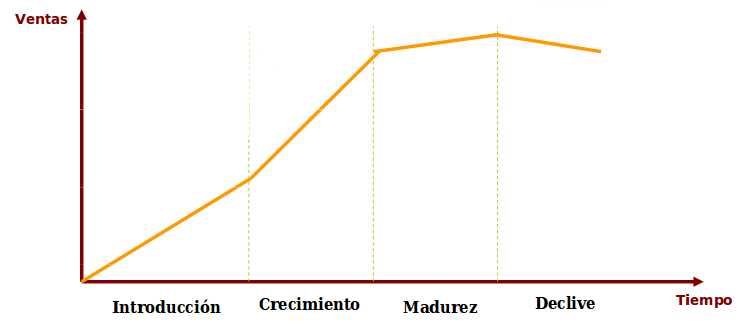
\includegraphics[width=0.8\textwidth]{2}
                              \caption{Ciclo de vida de un producto/servicio}
                              \label{vida_producto}
                        \end{figure}

                  \subsubsection{\textcolor[rgb]{0.9,0.7,0.6}Etapas en el desarrollo del producto}

                        El proceso de desarrollo de productos representa la secuencia básica de los pasos o actividades que la empresa sigue para diseñar y llevar el producto al mercado. En este proceso se deben tener en cuenta aspectos como:
                        \begin{enumerate}[1)]
                              \item Las tendencias de la demanda
                              \item Los costes de producción y la relación con los precios de venta
                              \item Las materias primas disponibles
                              \item Los procesos productivos y la tecnología disponibles
                              \item El impacto del nuevo producto sobre los productos ya existentes de la empresa
                              \item Nivel de calidad preciso
                        \end{enumerate}
                        
                        Teniendo esto en cuenta distinguimos cinco etapas en el desarrollo de un producto:
                        \begin{description}
                              \item[Generación de ideas]: se obtiene información sobre las necesidades y exigencias del mercado, identificando las oportunidades existentes. Las fuentes de generación de ideas pueden ser clientes, ingenieros, diseñadores, universidades, etc.

                              \item[Evaluación y selección]: las ideas generadas en la primera fase pasan por una serie de filtros. Se seleccionan aquellas ideas que presentan mayores posibilidades de éxito. Este proceso de evaluación implica un análisis de la viabilidad del producto desde diferentes puntos de vista:
                              \begin{enumerate}[---]
                                    \item \textit{\textcolor[rgb]{0.9,0.7,0.6}{Viabilidad comercial}}: consiste en analizar si existe un mercado para ese producto.
                                    \item \textit{\textcolor[rgb]{0.9,0.7,0.6}{Viabilidad económica}}: se realiza un análisis coste-beneficio que nos permita estimar si ese producto proporcionará un margen adecuado, teniendo en consideración su coste estimado de producción, así como el precio  al que podría venderse.
                                    \item \textit{\textcolor[rgb]{0.9,0.7,0.6}{Viabilidad técnica}}: es necesario comprobar que la empresa cuenta con la capacidad técnica y tecnológica adecuada para la fabricación en serie del producto.
                                    \item \textit{\textcolor[rgb]{0.9,0.7,0.6}{Valoración de las reacciones de la competencia}}: valorar la posible reacción de la competencia ante nuestro lanzamiento, ya que en algunas ocasiones nuestra empresa no contará con los recursos suficientes para una ``guerra abierta'' con nuestros competidores; en estos casos, quizá la estrategia más adecuada es no continuar con el proceso de diseño.
                                    \item \textit{\textcolor[rgb]{0.9,0.7,0.6}{Ajuste a los objetivos de la organización}}: los nuevos productos deben respetar la estrategia de la organización, contribuyendo a alcanzar los objetivos establecidos.
                              \end{enumerate}
                              \item[Desarrollo y diseño del producto y del proceso]: Se generan arquitecturas alternativas del producto, se decide sobre la geometría de las piezas, se identifica a los proveedores, se diseñan las máquinas, se estudia el diseño de los procesos para conseguir la calidad deseada, etc.
                              \item[Fabricación de prototipos y evaluación]: se realizan pruebas y evaluación correspondientes a los diseños resultantes de la tercera fase, para lo cual se procede a la fabricación de prototipos y a la simulación del proceso de fabricación, tratando de detectar posibles deficiencias. Posteriormente, se procede a la realización  de pruebas de mercado que permiten simular las condiciones reales del mercado con objeto de seleccionar la estrategia de lanzamiento más adecuada y realizar una previsión de la cifra de ventas.
                              \item[Lanzamiento del producto]: fabricación a gran escala. Si la evaluación realizada en la fase anterior es favorable, el producto pasa a la quinta fase, en la que se inicia la fabricación a gran escala; se produce el lanzamiento al mercado del nuevo producto, su distribución inicial y las operaciones de apoyo al mismo.
                        \end{description}

            \subsection{\textcolor[rgb]{0.9,0.7,0.6}Diseño del proceso productivo}

                  El proceso productivo está formado por un conjunto actividades coordinadas para realizar la producción con la determinación correcta de medios, de manera que se obtenga el producto con la máxima eficiencia, minimizando costes y tiempo. Hay cuatro estrategias de proceso existentes que se diferencian según la cantidad y la variedad de los productos fabricados:

                  \begin{description}
                        \item[Enfoque a proceso]: las configuraciones por proyectos están orientadas a la fabricación de un solo producto, hecho bajo pedido a medida. En las configuraciones productivas por lotes o talleres, los puestos de trabajo están agrupados por funciones y los productos van pasando por cada uno de los talleres hasta completar su procesamiento. La producción se realiza por lotes pequeños de una gran variedad de productos. Estos procesos tienen un alto grado de flexibilidad de producto y la producción es a medida. Sin embargo, los talleres presentan una tasa de utilización muy baja. Para evitar esto último y reducir las listas de espera, será necesario realizar una correcta programación de pedidos y establecer las prioridades de entrada de éstos a los talleres.

                        \item[Enfoque repetitivo]: también llamado por módulos. Los módulos son un conjunto de componentes preparados previamente. Los módulos pueden ser combinados para obtener múltiples resultados y, de esta forma, obtener un producto casi a medida para el cliente. Son menos flexibles pero son más eficientes.

                        \item[Enfoque a producto]: también llamado de fabricación continua. Se caracteriza por la fabricación de grandes volúmenes de una reducida variedad de productos. Se ejecutan siempre las mismas operaciones, en las mismas máquinas, se obtiene el mismo producto y las máquinas estarán dispuestas en cadena. Se mejora el flujo de materiales y trabajo, consiguiendo una alta especialización y destreza en los trabajadores. Este enfoque es recomendable cuando la demanda es uniforme y se trata de un producto estandarizado.

                        \item[Personalización en masa]: está orientado a dar mayor valor añadido a los clientes, simultaneando sistemas de producción de grandes volúmenes, muy eficientes en costes y personalizados a las necesidades de cada cliente.
                  \end{description}

            \subsection{\textcolor[rgb]{0.9,0.7,0.6}Planificación de la capacidad productiva}

                  Se entiende por \textit{\textcolor[rgb]{0.9,0.7,0.6}{capacidad productiva}} el máximo nivel de producción que puede ofrecer una estructura económica determinada. La capacidad productiva se expresa por medio de unidades que pueden obtenerse en relación a un período de tiempo.

                  La capacidad de producción indica si somos capaces de atender la demanda o si las instalaciones y equipos permanecerán inactivos. Lo ideal es que la estructura permita tener una capacidad productiva flexible que nos permita adaptarnos a variaciones de los niveles de producción.

                  La planificación de la capacidad se puede realizar desde un horizonte temporal a largo, medio y corto plazo.
                  \begin{enumerate}[---]
                        \item En la planificación a largo plazo, la empresa puede tomar deciciones de carácter estructural e incluso realizar inversiones sobre las instalaciones y equipos. 
                        \item En el medio plazo, la empresa puede adaptar su capacidad a través de las contrataciones/despidos de personal, con horas extras, subcontratación, etc.
                        \item En el corto plazo, la adaptación de la capacidad de la empresa a las exigencias del mercado es mucho más difícil. En estos casos se podría recurrir a modificar los programas de trabajo o reasignar cargas de trabajo.
                  \end{enumerate}

                  \subsubsection{\textcolor[rgb]{0.9,0.7,0.6}Tipos de capacidad productiva}

                        \begin{description}
                              \item[Capacidad proyectada o diseñada]: tasa de producción ideal para la cual se diseñó el sistema
                              \item[Capacidad efectiva o real]: capacidad que espera alcanzar una empresa según sus actuales limitaciones operativas.
                        \end{description}

                        Relacionado con el nivel de aprovechamiento de la capacidad de la empresa, aparecen dos conceptos:
                        \begin{enumerate}[---]
                              \item \textit{\textcolor[rgb]{0.9,0.7,0.6}{Tasa de utilización}}: porcentaje alcanzado de la capacidad proyectada.
                              \begin{equation}
                                    \txt{Utilización}=\frac{\txt{salida real}}{\txt{cap. proyectada}}\ast100\%
                              \end{equation}
                              \item \textit{\textcolor[rgb]{0.9,0.7,0.6}{Tasa de eficiencia}}: porcentaje de la capacidad efectiva alcanzada realmente.
                              \begin{equation}
                                    \txt{Eficiencia}=\frac{\txt{salida real}}{\txt{cap. efectiva}}\ast100\%
                              \end{equation}
                        \end{enumerate}

            \subsection{\textcolor[rgb]{0.9,0.7,0.6}Decisión de localización}

                  La importancia de las decisiones de localización en la empresa vienen justificadas por dos razones principalmente:
                  \begin{enumerate}[1.]
                        \item Porque suponen importantes inmovilizaciones financieras a largo plazo
                        \item Por su influencia directa en la capacidad competitiva de la empresa
                  \end{enumerate}

                  La localización de una empresa afecta tanto a los costes fijos como a los costes variables. La frecuencia con la que se toman este tipo de decisiones dependerá del tipo de negocio.

                  Las causas que pueden obligar a una empresa a tomar decisiones sobre su localización son:
                  \begin{enumerate} [1.]
                        \item Mercado en expansión
                        \item Introducción de nuevos productos
                        \item Contracción de la demanda
                        \item Agotamiento de las fuentes de abastecimiento
                        \item Obsolescencia de una planta de fabricación
                        \item Cambios en las condiciones políticas o económicas de la región donde está ubicada
                        \item Fusiones o adquisiciones entre empresas.
                  \end{enumerate}

                  Las alternativas de localización pueden ser de tres tipos:
                  \begin{enumerate}[1º]
                        \item Expandir una instalación existente
                        \item Crear nuevas instalaciones en nuevos lugares
                        \item Cerrar instalaciones en algún lugar y abrir otras en otro(s) sitio(s)
                  \end{enumerate}

                  La globalización de los mercados ha supuesto una mayor complejidad a la hora de decidir la localización de la empresa. Los factores que pueden condicionar este tipo de decisiones están relacionados con:
                  \begin{enumerate}
                        \item Fuentes de abastecimiento
                        \item Localización de los mercados
                        \item Costes
                        \item Tipo de comunicaciones
                        \item Riesgos políticos
                        \item Atractivos de la zona
                        \item Condiciones climatológicas
                        \item Impuestos
                        \item Marco jurídico
                  \end{enumerate}

            \subsection{\textcolor[rgb]{0.9,0.7,0.6}Distribución en planta o estrategia de layout}

                  Con el proceso de distribución en planta se pretende determinar la mejor ordenación de los factores disponibles, de modo que constituyan un sistema productivo capaz de alcanzar los objetivos fijados de la forma más adecuada y eficiente posible. Para ello es imprescindible contar con equipos ligeros, móviles y flexibles y personal polivalente.

                  Los principales objetivos que se persiguen con una adecuada distribución en planta son:
                  \begin{enumerate} [---]
                        \item Mejorar el aprovechamiento del espacio, equipo y personas
                        \item Mejorar el flujo de información, materiales y personas
                        \item Mejorar la moral y la seguridad de las condiciones de trabajo de los empleados
                        \item Mejorar la interacción con el cliente
                        \item Mayor flexibilidad
                  \end{enumerate}

                  La distribución en planta de una empresa dependerá del tipo de producto fabricado y el nivel de demanda que se pretenda atender. Los tipos de distribución en planta son:

                  \begin{description}
                        \item[Distribución en planta enfocada al proceso]: está indicado cuando se produce un bajo volumen de una alta variedad de productos
                        \item[Distribución en planta enfocada al producto]: se utiliza cuando la producción es continua
                        \item[Distribución en planta en línea]: es una distribución en planta intermedia, entre un enfoque a producto y un enfoque a proceso. Funciona por módulos y es indicada para líneas de ensamblaje.
                  \end{description}

      \section{\textcolor[rgb]{0.9,0.7,0.6}Decisiones tácticas de operaciones}

            \subsection{\textcolor[rgb]{0.9,0.7,0.6}Cadena de suministro}

                  El objetivo de la dirección de la cadena de suministro es integrar y sincronizar los flujos de materiales, los servicios y la información que se producen con los proveedores y con los clientes. La gestión de la cadena de suministros busca racionalizar la base de proveedores, reducir los inventarios de la cadena, reducir tiempos de espera y de respuesta, disminuir costes de obsolescencia de la cadena, reducir el tiempo al mercado o sincronizar la programación que se realiza entre empresas.

                  Cuando se diseña la cadena de suministro, para que ésta sea eficiente es importante establecer la forma en que los materiales y los productos se van desplazar desde los proveedores a las plantas de transformación, desde éstas a los distribuidores y desde éstos a los clientes. Atendiendo a estos desplazamientos, vamos a diferenciar dos movimientos: los que se producen desde cada uno de los proveedores hasta la empresa creadora del bien o servicio, que serían las compras o aprovisionamiento de los materiales, y los que se producen desde la empresa que obtiene el producto terminado hasta el cliente final, que se refieren a la distribución de los productos.

                  \begin{description}
                        \item[La función de compras] supone decidir qué materiales y suministros se utilizarán, lo cual implica también identificar a los proveedores que van a suministrar los artículos a la empresa. Será necesario decidir si producir o comprar.

                        \item[La función de distribución] consiste en administrar los flujos de productos desde los fabricantes hasta los clientes, lo cual incluye actividades de almacenamiento y de transporte. El valor añadido que se le aporta al producto es el tiempo y el lugar en que está disponible.
                  \end{description}

                  Con la gestión de inventarios se pretende dar respuesta a dos cuestiones fundamentales del proceso productivo:
                  \begin{enumerate}
                        \item Cuánto pedir de cada producto, para mantener un nivel de existencias adecuado y poder atender correctamente la demanda.

                        \item Cuándo realizar los distintos pedidos, para cubrir las necesidades de producción
                  \end{enumerate}

                  La respuesta a estas preguntas se obtiene con una serie de técnicas de la gestión de inventarios:

                  \begin{description}
                        \item[Técnicas clásicas de gestión de inventarios]: se suelen utilizar cuando la demanda es independiente, es decir, cuando las fluctuaciones de la demanda dependen directamente de las condiciones del mercado. Persiguen la minimización de los costes totales que intervienen en la gestión de inventarios.

                        \item[La planificación de las necesidades de materiales (MRP)]: esta técnica se utiliza cuando la demanda es dependiente. Es decir, cuando la demanda de un artículo depende de la demanda de otro u otros artículos más complejos. En estos casos, la demanda es conocida y cierta. Persigue reducir los niveles de inventario y, por tanto, los costes de almacenamiento. Persigue también dar un mejor servicio al cliente, en cuanto a entrega de pedidos en fecha, calidad y cantidad.
                  \end{description}

\chapter{\textcolor[rgb]{0.4,0.7,0.4}La dirección financiera}
      
    \section{\textcolor[rgb]{0.4,0.7,0.4}La dirección financiera y sus objetivos}

        La dirección financiera se encarga de todas las decisiones de inversión y de financiación que se llevan a cabo dentro de la empresa. Es importante resaltar que mientras las oportunidades con las que cuenta la empresa para invertir son casi infinitas, los recursos financieros para llevarlos a cabo no, por ello, aunque la decisión de invertir está muy relacionada con la rentabilidad que se espera obtener, la inversión estará limitada por la capacidad financiera de la empresa. Por ello, la inversión y la financiación están muy relacionadas hasta el punto de conseguir que la rentabilidad de las inversiones sea mayor al coste de financiación de las mismas.

        Los principales objetivos de la dirección financiera pueden concretarse en los siguientes:
        \begin{enumerate}
            \item Utilizar de forma óptima los recursos financieros.
            \item Analizar la mejor manera posible de financiar los proyectos de inversión elegidos.
            \item Determinar el punto de equilibrio financiero de la empresa.
        \end{enumerate}

    \section{\textcolor[rgb]{0.4,0.7,0.4}El balance}

        La fotografía de la empresa en relación a la inversión y financiación en un momento determinado del tiempo (enfoque \textbf{estático}) se muestra en el \textit{\textcolor[rgb]{0.4,0.7,0.4}{balance}}:
        \begin{center}
            \begin{tabular}{|p{4cm}|p{4cm}|}
                \hline
                \rowcolor[rgb]{0.4,0.7,0.4} \textbf{Estructura económica o activo} & \textbf{Estructura financiera} \\
                \hline
                Empleo dado a los recursos conseguidos por la empresa & Origen de los recursos financieros conseguidos por la empresa \\
                \hline
                Recoge los elementos que la empresa tiene que adquirir para el desarrollo de su actividad & Los recursos financieros que la empresa capta para poder realizar sus inversiones \\
                \hline
                Activo no corriente (inmovilizado) y corriente & Los recursos financieros que la empresa capta para poder realizar sus inversiones \\
                \hline
                \hline
                \multicolumn{2}{|p{8cm}|}{Importe de la estructura económica = Importe de la estructura financiera (pues necesitan estar equilibrados)} \\
                \hline
                \end{tabular}
            \end{center}

    \section{\textcolor[rgb]{0.4,0.7,0.4}La inversión}

        La inversión se define como la materialización de los recursos financieros en bienes de consumo y de equipo. En sentido estricto, se entiende por inversión todos los desembolsos destinados a la adquisición de bienes de inmovilizado aunque en un sentido más amplio también abarca la adquisión de mercancías, materiales, etc.

        Estas inversiones están reflejadas en el activo del balance, el cual está dividido atendiendo al tiempo que permanecen los elementos en la empresa: el activo corriente y el no corriente:
        \begin{description}
            \item[Activo no corriente]: se compone de las \textit{\textcolor[rgb]{0.4,0.7,0.4}{inversiones de estructura}} que permanecen en la empresa por un período de tiempo superior a un ejercicio económico (un año).
            \item[Activo corriente]: se compone de las \textit{\textcolor[rgb]{0.4,0.7,0.4}{inversiones de funcionamiento}} que permanecen en la empresa por un período de tiempo inferior al ejercicio económico y que se recuperan a través de su proceso productivo. El activo corriente se puede desagregar a su vez en:
            \begin{enumerate}
                \item Existente.
                \item Deudores comerciales, otras cuentas a cobrar e inversiones a corto plazo.
                \item Efectivo y otros activos líquidos equivalentes.
            \end{enumerate}
        \end{description}

      \subsection{\textcolor[rgb]{0.4,0.7,0.4}Los ciclos de la inversión de la empresa}

            Dentro de las inversiones que se pueden acometer en la empresa también se puede distinguir entre aquéllas que se recuperan a través de un ciclo a corto plazo y a un ciclo a largo plazo:
            \begin{description}
                \item[Ciclo a largo plazo]: dentro de las inversiones que forman parte del \textbf{ciclo a largo plazo} se distinguen aquéllos activos no corrientes que son amortizables (por ej, edificios) y aquellos que no son amortizables (por ej, solares). Mediante el cálculo del período medio de permanencia de ambos tipos de inmovilizados en la empresa se obtendrá una estimación de la duración del ciclo a largo plazo de la empresa.

                \item[Ciclo a corto plazo]: se denomina \textit{\textcolor[rgb]{0.4,0.7,0.4}{período medio de maduración}}, el cual se define como el tiempo que por término medio tarda en volver a caja el dinero que ha salido de la empresa para hacer frente a exigencias de la actividad productiva. En el caso de empresas dedicadas a la fabricación y comercialización de productos, el período medio de maduración está compuesto por los siguientes subperíodos:
                \begin{enumerate}
                    \item Período medio de aprovisionamiento.
                    \item Período medio de fabricación ($PM_{fa}$).
                    \item Período medio de venta ($PM_{v}$).
                    \item Período medio de cobro ($PM_{c}$).
                \end{enumerate}
                En el caso de que la empresa obtenga un aplazamiento de pago por parte de sus proveedores, puede distinguirse entre \textit{\textcolor[rgb]{0.4,0.7,0.4}{período medio de maduración económico}} ($PMM_{e}$) y \textit{\textcolor[rgb]{0.4,0.7,0.4}{período medio de maduración financiero}} ($PMM_{f}$). $PM_{p}$ es el período medio de pago.
            \end{description}
            \begin{center}
                \textbf{Diferencia entre período medio de maduración económico y financiero} \\
                \framebox[1.1\width]{$PMM_{e} = PM_{a} + PM_{fa} + PM_{v} + PM_{c}$} \par
                \framebox[1.1\width]{$PMM_{f} = PM_{a} + PM_{fa} + PM_{v} + PM_{c} - PM_{p}= PMM_{e} - PM_{p}$} \par
            \end{center}
        \newpage      
        \subsection{\textcolor[rgb]{0.4,0.7,0.4}Factores a considerar para llevar a cabo la inversión en la empresa}

            \begin{description}
                  \item[La rentabilidad]:  es el factor clave para valorar un proyecto de inversión y se define como \textit{\textcolor[rgb]{0.4,0.7,0.4}{la medida en términos relativos del beneficio que obtiene la empresa}}. El análisis de las inversiones está basado en una medida más objetiva, concretamente los flujos de dinero líquido, si en lugar de evaluar la diferencia entre ingresos y costes se consideran los cobros y pagos, se elimina el efecto subjetivo que supone la determinación del beneficio.
                  \begin{center}
                        $\txt{Rentabilidad} = \frac{\txt{Beneficio}}{\txt{Inversión}}$
                  \end{center}

                  \item[El valor del dinero en el tiempo]:
                  \begin{enumerate}
                        \item \textbf{La pérdida de poder adquisitivo}: si se inmoviliza un dinero ahora se espera obtener una ganancia futura superior que tenga, al menos, el mismo poder adquisitivo que la actual
                        \item \textbf{El coste de oportunidad}: no recibir dinero ahora elimina la posibilidad de invertirlo en un proyecto que genere ganancias
                  \end{enumerate}
            \end{description}

      \subsection{\textcolor[rgb]{0.4,0.7,0.4}Las variables de la inversión desde un punto de vista financiero}

            Las variables de las que se compone cualquier proyecto de inversión son:
            \begin{description}
                  \item[Desembolso inicial] ($A_{0}$): el pago que origina la adquisión de elementos del activo.
                  \item[El horizonte temporal de la inversión] ($n$): período de tiempo desde que se hace efectivo el desembolso inicial hasta que se producen los últimos cobros o/y pagos de la inversión.
                  \item[El flujo neto de caja o cash-flow de tesorería] ($Q_{j}$): representa las entradas o cobros ($C_{j}$) y salidas o pagos ($P_{j}$) de dinero líquido que se producen en cada uno de los períodos del proyecto de inversión:
                  \begin{center} 
                        $Q_{j} = C_{j} - P_{j}$ 
                  \end{center}
            \end{description}

      \subsection{\textcolor[rgb]{0.4,0.7,0.4}Métodos de selección de inversores}

            Existe una amplia variedad de métodos que pueden usarse para seleccionar cuáles son las inversiones que aportan un mayor valor a la empresa, dividiéndose éstos en dos grandes grupos:
            \begin{description}
                  \item[Métodos estáticos]: se omite la influencia del valor del dinero en el tiempo.
                        \begin{enumerate}
                              \item Criterio del flujo neto de caja total.
                              \item Criterio del plazo de recuperación o \textit{\textcolor[rgb]{0.4,0.7,0.4}{``pay-back''}} estático.
                        \end{enumerate}
                  \item[Métodos dinámicos]: exigen que las magnitudes monetarias sean homogéneas, es decir, que estén referidas todas ellas a un mismo momento del tiempo.
                        \begin{enumerate}
                              \item El criterio del plazo de recuperación o \textit{\textcolor[rgb]{0.4,0.7,0.4}{``pay-back''}} dinámico.
                              \item Criterio del valor actual neto (VAN).
                              \item Criterio de la tasa interna de rentabilidad (TIR).
                        \end{enumerate}
            \end{description}

      \section{\textcolor[rgb]{0.4,0.7,0.4}La financiación: estructura financiera}

            El activo o estructura económica de la empresa está constituido por el conjunto de bienes y derechos que necesita una empresa para llevar a cabo su actividad. La empresa debe disponer de los recursos monetarios necesarios para poder adquirir esos elementos que componen la inversión. Se conocen como recursos financieros o fuentes de financiación, y engloban el conjunto de deudas y obligaciones que debe satisfacer una empresa, los recursos financieros aparecen bajo la denominación de \textit{\textcolor[rgb]{0.4,0.7,0.4}{patrimonio neto}} y \textit{\textcolor[rgb]{0.4,0.7,0.4}{pasivo}}.

            La financiación obtenida por la empresa en el transcurso de su actividad económica es uno de los aspectos más importantes que los directivos deben tener en cuenta con el fin de conseguir la supervivencia o el crecimiento de la misma a lo largo del tiempo. No sólo será relevante determinar la cantidad óptima de recursos que va a necesitar la empresa para financiar su estructura económica, sino que también va a ser imprescindible que la obtención de esa financiación se consiga en las mejores condiciones posibles.

            \subsection{\textcolor[rgb]{0.4,0.7,0.4}Estructura financiera según la propiedad de los recursos financieros}

                  \begin{description}
                        \item[Recursos propios]: están constituidos por aquellos recursos financieros aportados directamente a la empresa por sus socios o propietarios (\textit{\textcolor[rgb]{0.4,0.7,0.4}{capital social}}), más la parte de los beneficios obtenidos por la empresa en los diferentes ejercicios económicos que no han sido distribuidos entre sus socios en forma de dividendos (\textit{\textcolor[rgb]{0.4,0.7,0.4}{reservas}}). Los recursos propios se caracterizan por ser la fuente de financiación más estable de la empresa, ya que no es necesario devolverlos en un plazo determinado y la empresa no tiene que pagar un tipo de interés por su utilización.
                        \item[Recursos ajenos]: son los recursos financieros que la empresa obtiene del exterior. Se caracterizan por que la empresa sí tiene la obligación de devolverlos en un plazo determinado y debe asumir un determinado coste por su utilización.
                  \end{description}

            \subsection{\textcolor[rgb]{0.4,0.7,0.4}Estructura financiera según el tiempo de vinculación de los recursos financieros}

                  \begin{description}
                        \item[Recursos permanentes]: formados por aquellos recursos financieros utilizados por la empresa que, o bien no tiene la obligación de devolverlos (\textit{\textcolor[rgb]{0.4,0.7,0.4}{patrimonio neto}}), o teniendo la obligación de devolverlos su plazo de devolución es superior a un año (\textit{\textcolor[rgb]{0.4,0.7,0.4}{pasivo no corriente}}). Dentro del patrimonio neto se incluyen los recursos propios.
                        \item[Pasivo corriente]: constituido por los recursos financieros que la empresa debe devolver en un plazo de tiempo inferior o igual a un año (\textit{\textcolor[rgb]{0.4,0.7,0.4}{recursos ajenos a corto plazo}}).
                  \end{description}

            \subsection{\textcolor[rgb]{0.4,0.7,0.4}Estructura financiera según el origen de los recursos}

            	\begin{description}
            		\item[Financiación interna o autofinanciación]: formada por los recursos financieros que son generados en el interior de la propia empresa. Se incluyen en esta modalidad las reservas (autofinanciación por enriquecimiento o neta), las amortizaciones y deterioros de valor (autofinanciación por mantenimiento). 

            		\item[Financiación externa]: formada por los recursos financieros que son son generados por la empresa. Se incluyen en esta modalidad el capital social, la prima de emisión de acciones\footnote{La prima de emisión de acciones está formada por las aportaciones directas que hacen los accionistas que adquieren nuevas acciones de la empresa cuando se produce una ampliación de capital con un valor de emisión superior a su valor nominal} y los recursos ajenos tanto a corto como a largo plazo.
            	\end{description}
            	
            	\subsubsection{\textcolor[rgb]{0.4,0.7,0.4}La financiación interna o autofinanciación}

            		Puede ser de dos tipos: enriquecimiento o mantenimiento:

            		\begin{description}
            			\item[La autofinanciación de mantenimiento]: \textbf{La amortización técnica}: su objetivo es mantener la capacidad productiva de la empresa, procediendo a la renovación de los activos no corrientes conforme se van deteriorando o van quedando obsoletos. La amortización técnica se define como la cuantificación en términos monetarios de la depreciación o pérdida de valor, que, por diversas razones, sufren los elementos de activo no corriente. Esta depreciación puede ser física, por obsolescencia, o por agotamiento o caducidad.

            			\item[La autofinanciación de enriquecimiento]: \textbf{La autofinanciación de enriquecimiento de reservas}: Su objetivo es financiar proyectos de inversión que permitan aumentar la capacidad productiva de la empresa. Las reservas se constituyen por la parte del beneficio obtenido por la empresa y que no es distribuido entre sus socios o propietarios en forma de dividendos. Hay varios tipos de reservas:
            			\begin{enumerate}
            				\item Reservas legales (se constituyen por ley)
            				\item Reservas voluntarias (se constituyen libremente por la empresa)
            				\item Reservas especiales (se establecen por cualquier disposición legal con carácter obligatorio pero son distintas a las legales).
            			\end{enumerate}
            			Las principales ventajas de la autofinanciación por enriquecimiento son:
            			\begin{enumerate}
            				\item Mayor autonomía financiera de la empresa
            				\item La empresa no tiene que pagar ningún coste por su utilización
            				\item Para empresas con poca o con nula capacidad de endeudamiento, es prácticamente la única fuente de financiación que pueden utilizar
            			\end{enumerate}
            			Y los inconvenientes son:
            			\begin{enumerate}
            				\item Son recursos financieros que se generan de forma discontinua, ya que dependen de la obtención de beneficios por parte de la empresa.
            				\item Puesto que el coste del uso de estos recursos es nulo para la empresa, se puede caer en el error de invertirlos de forma inapropiada en proyectos de inversión de escasa rentabilidad.
            			\end{enumerate}
            		\end{description}

    \section{\textcolor[rgb]{0.4,0.7,0.4}El equilibrio financiero de la empresa}

    	La situación de equilibrio financiero de la empresa es aquella en la que los elementos del activo no corriente se financien con recursos cuyo plazo de devolución sea también largo (recursos permanentes) y que los elementos del activo corriente se financien con recursos cuyo plazo de devolución sea también corto (pasivo corriente), sin embargo, la empresa debe conseguir que sus capitales permanentes sean superiores a la cantidad necesaria para financiar no sólo el activo no corriente, sino también una parte del activo corriente para  evitar una situación de insolvencia técnica o suspensión de pagos. A este excedente se lo conoce como \textit{\textcolor[rgb]{0.4,0.7,0.4}{fondo de maniobra}} y constituye una especie de fondo de previsión que permite a la empresa hacer frente a desfases temporales que se puedan producir entre pagos y cobros procedentes de un ciclo de explotación.
    	\newpage
    	\[\begin{xy}
            ,(0,0)*+=[]=<1.5cm>[]\txt<1.5cm>{Activo}
            ,(0,-10)*+=[]=<1.5cm>[F]\txt<1.5cm>{Activo no corriente}
            ,(0,-25)*+=[]=<1.5cm>[F]\txt<1.5cm>{Activo corriente}
            ,(50,0)*+=[]=<1.5cm>[]\txt<1.5cm>{Pasivo}
            ,(50,-10)*+=[]=<1.5cm>[F]\txt<1.5cm>{Recursos permanentes}
            ,(50,-25)*+=[]=<1.5cm>[F]\txt<1.5cm>{Pasivo corriente}
            ,(0, -40)*+=[]=<1.5cm>[]\txt<1.5cm>{Activo}
            ,(0, -50)*+=[]=<1.5cm>[F]\txt<1.5cm>{Activo no corriente}
            ,(0, -65)*+=[]=<1.5cm>[F]\txt<1.5cm>{Activo corriente}
            ,(50,-40)*+=[]=<1.5cm>[]\txt<1.5cm>{Pasivo}
            ,(50,-50)*+=[]=<1.5cm>[F]\txt<1.5cm>{Recursos permanentes}
            ,(50,-65)*+=[]=<1.5cm>[F]\txt<1.5cm>{Activo corriente}
            ,(20,-50)*+=[]=<1.5cm>[]\txt<1.5cm>{Fondo maniobra}
            \ar@{-} (5,-17.5);(55,-17.5)
            \ar@{-} (5,-57.5);(55,-57.5)
    	\end{xy}\]

    	Como se puede apreciar en la figura anterior, el fondo de rotación puede calcularse de tres formas:
    	\begin{enumerate}[---]
    		\item Diferencia entre activo corriente y pasivo corriente
    		\item Diferencia entre recursos permanentes y activo no corriente
    		\item Suponiendo que el activo no corriente está financiado íntegramente con recursos permanentes, el fondo de rotación es la parte del activo corriente que se financia con recursos permanentes
    	\end{enumerate}

\chapter{\textcolor[rgb]{0.8,0.2,0.8}La dirección de recursos humanos}

      \section{\textcolor[rgb]{0.8,0.2,0.8}Introducción a la dirección de recursos humanos}

            La función de recursos humanos ha sido denostada frente a otras funciones y considerada tradicionalmente como una función secundaria o incluso sin importancia. Más recientemente, se está demostrando que su importancia es mucho mayor de la estimada históricamente y se está equiparando al resto de funciones.

            La dirección de recursos humanos, se puede definir como la atracción, selección, retención, desarrollo y utilización de los recursos humanos para conseguir los objetivos de la organización.

      \section{\textcolor[rgb]{0.8,0.2,0.8}Las funciones principales de la dirección de recursos humanos}

            La función de recursos humanos se suele subdividir a su vez en las siguientes subfunciones:
            \begin{enumerate}
                  \item Planificación
                  \item Reclutamiento
                  \item Selección
                  \item Compensación
                  \item Evaluación de personal
                  \item Desarrollo y formación
                  \item Relaciones laborales
                  \item Seguridad e higiene en el trabajo
            \end{enumerate}

            \subsection{\textcolor[rgb]{0.8,0.2,0.8}Planificación de recursos humanos}

                  Los objetivos y estrategias sólo pueden alcanzarse y desarrollarse cuando la organización dispone de personas con las capacidades, habilidades, conocimientos y actitudes necesarias y adecuadas para llevarlas a cabo.

                  La planificación de recursos humanos se encarga de comprobar lo anterior mediante la revisión sistemática de las necesidades de recursos humanos de la empresa, con el fin de asegurar que el número requerido de empleados, con las habilidades requeridas esté disponible para cuando se necesita.

                  El análisis de puestos consiste en la exploración y análisis de las tareas que componen un puesto de trabajo, así como en la descripción de las habilidades requeridas para ocupar el puesto de forma adecuada, y de las responsabilidades que conlleva.

                  El análisis y descripción de puestos no sólo se utiliza en la planificación de recursos humanos, sino que constituye la principal herramienta para otras subfunciones de recursos humanos, como la formación.

                  El pronóstico de necesidades de recursos humanos puede ser complicado, pero existen herramientas, como la técnica Delphi, que ayudan a establecer la futura demanda de recursos humanos de la organización. También existen técnicas que permiten el análisis y revisión de los recursos humanos actuales, como el ``inventario de capacidades'' de los empleados. Para decidir cómo conseguir lo que la organización necesita, hay distintas opciones y van desde acudir al mercado laboral, promocionar a empleados actuales hasta los despidos, etc.

                  \subsubsection{\textcolor[rgb]{0.8,0.2,0.8}Desarrollo de la carrera profesional}

                        Consiste en intentar alinear las metas profesionales de los empleados con los objetivos y necesidades de la planificación de recursos humanos de una empresa. De esta forma, la organización ofrece a sus empleados generalmente en puestos directivos, el apoyo para conseguir metas de carrera realistas y las oportunidades de relizarlas.

                        Es una práctica más extendida entre las grandes empresas. Su principal ventaja es asegurarse la disposición de un grupo de personas cualificadas que permitan satisfacer las necesidades futuras de recursos humanos. Otras ventajas que se pueden ofrecer son:
                        \begin{enumerate}
                              \item Uso eficaz del personal
                              \item Reducción del absentismo
                              \item Reducción de la tasa de abandono
                              \item Mejora de la moral y del clima laboral
                              \item Menor posibilidad de obsolescencia de conocimientos
                              \item Mayor nivel de flexibilidad de los trabajadores
                              \item Mayor número de candidatos válidos para una promoción
                              \item Mejora de la imagen de la empresa, que conlleva un mayor número de candidatos quieran trabajar en ella.
                        \end{enumerate}
	     
           \subsection{\textcolor[rgb]{0.8,0.2,0.8}Reclutamiento}

                  El proceso de reclutamiento recoge un conjunto de actividades orientadas a atraer al mayor número posible de candidatos válidos.

                  Existen factores tanto externos como internos que influyen en esta función de recursos humanos:
                  \begin{description}
                        \item[Factores externos]: oferta de mano de obra, suministro de habilidades en el mercado laboral, consideraciones legales, etc.
                        \item[Factores internos]: la política de promoción interna de la empresa, como por ejemplo la imagen corporativa o reputación que la empresa tenga o pretenda crear, la cultura medioambiental de la empresa, etc.
                  \end{description}

                  Los métodos de reclutamiento son variados: publicidad, páginas web especializadas, programas-contratos con universidades, página web corporativa, eventos especiales, solicitudes espontáneas, etc.

            \subsection{\textcolor[rgb]{0.8,0.2,0.8}Selección}

                  La selección es una actividad restrictiva que pretende elegir, de entre los candidatos posibles, aquél más idóneo, capaz de integrarse en la empresa y desempeñar las tareas que se le asignen.

                  Las técnicas de selección del personal que se utilizan más habitualmente son: test o pruebas psicotécnicas, pruebas profesionales o de conocimiento, pruebas de eficiencia, simulaciones, entrevistas, etc.

            \subsection{\textcolor[rgb]{0.8,0.2,0.8}Compensación}

                  La compensación más obvia es la económica, sin embargo, existen otras ``compensaciones'', como promociones laborales o asignaciones de las tareas más deseables o la aceptación de los compañeros de trabajo, buen ambiente laboral, reconocimiento del superior, etc.

                  La compensación, como intercambio o relación económica, es aquella que compensa o retribuye al empleado por realizar las labores asignadas y todo lo que conlleva la correcta utilización de éstas. Su objetivo principal es atraer, retener y motivar a los recursos humanos para que realicen las tareas asignadas de la forma adecuada.

                  Esta subfunción de compensación recoge todas las decisiones, procesos y prácticas relacionados con la gestión de la compensación.

                  La retribución total de un empleado incluye tres elementos:
                  \begin{description}
                        \item[Salario base]: cantidad fija que recibe normalmente el empleado
                        \item[Incentivos salariales]: programas diseñados para recompensar a los empleados con altos niveles de rendimiento
                        \item[Prestaciones o retribuciones indirectas]: incluyen gran variedad de programas, seguros médicos, vacaciones, etc. Un grupo importante son las \textit{\textcolor[rgb]{0.8,0.2,0.8}{retribuciones en especie}}.
                  \end{description}

            \subsection{\textcolor[rgb]{0.8,0.2,0.8}Evaluación del personal}

                  Es el proceso a través del cual se realiza un análisis de las capacidades y potencial de un empleado o futuro empleado. Los posibles usos de la evaluación personal son:
                  \begin{enumerate}[a)]
                        \item \textbf{Desarrollo}: indica qué empleados necesitan formación, facilita la valoración de la eficacia de los programas de formación y puede facilitar la detección de los aspectos de la relación entre supervisor-subordinado a mejorar.
                        \item Establecimiento de incentivos
                        \item Motivación
                        \item Planificación de recursos humanos
                        \item Compensación
                        \item Comunicación
                  \end{enumerate}

                  Para el establecimiento de un proceso de evaluación formal se aconseja que se sigan los siguientes pasos:
                  \begin{enumerate}[1.]
                        \item Establecimiento de estándares para cada puesto y los criterios para su evaluación.
                        \item Comunicación a los futuros evaluados de las expectativas
                        \item Determinar la periodicidad en la evaluación, cuándo, cómo, dónde se va a realizar y quién va a llevarla a cabo
                        \item Implementación del proceso de evaluación
                        \item Discutir los resultados de la evaluación con el evaluado.
                        \item Toma de acciones correctivas
                  \end{enumerate}

            \subsection{\textcolor[rgb]{0.8,0.2,0.8}Desarrollo de recursos humanos}

                  Este concepto recoge los procesos y actividades de formación y desarrollo para lograr un incremento o mejora en las habilidades, conocimientos, capacidades, actitudes, comportamientos, etc., de los trabajadores de la organización.

                  Se busca que el personal obtenga la información, los conocimientos y habilidades que necesita para desempeñar su puesto actual y los futuros, así como facilitar las herramientas necesarias para conseguirlo y el estímulo y motivación al personal para aprovechar la formación y utilizarla.

                  Las principales actividades de recursos humanos que se pueden englobar en el desarrollo de los recursos humanos son:

                  \subsubsection{\textcolor[rgb]{0.8,0.2,0.8}Orientación}

                        Recoge las actividades por las cuales se proporciona a los nuevos empleados la información necesaria para desempeñar su trabajo de forma correcta. Ésta complementa la ya recibida en el proceso de reclutamiento y selección, e incluye información sobre los siguientes aspectos:
                        \begin{enumerate}
                              \item Propia organización
                              \item Puesto de trabajo
                              \item Centro de trabajo, departamento, unidad, supervisores, subordinados, compañeros, y otros puestos de trabajo/empleados con los que tendrá que interactuar
                        \end{enumerate}

                  \subsubsection{\textcolor[rgb]{0.8,0.2,0.8}Socialización}

                        Su objetivo es facilitar la adaptación del trabajador a las nuevas circunstancias ante un cambio en el puesto de trabajo, lugar, etc.

                  \subsubsection{\textcolor[rgb]{0.8,0.2,0.8}Formación}

                        Engloba los métodos para proporcionar a los empleados conocimientos, habilidades y capacidades necesarias para desarrollar o aumentar el rendimiento en su actual o futuro puesto de trabajo, así como lograr un cambio en aspectos como la motivación, para la mejora del desempeño del trabajador.

                        Las técnicas de capacitación o formación son: la capacitación en el puesto, simuladores, juegos de rol, asesoramiento, videoconferencias, cursos a distancia, etc.

            \subsection{\textcolor[rgb]{0.8,0.2,0.8}Relaciones laborales}

                  Se refieren a las relaciones entre los trabajadores y la empresa, con el fin de establecer las normas básicas que rigen las relaciones del trabajo y facilitar la reducción de conflictos.

                  Recoge procesos de negociación colectiva, diversas formas de participación de los trabajadores y mecanismos de resolución de conflictos colectivos e individuales.

                  Los procesos de negociación colectiva se concretan en los denominados convenios colectivos. Un convenio colectivo es un acuerdo suscrito entre los representantes de los trabajadores y de los empresarios, sobre las condiciones laborales y las relativas a la remuneración del trabajo en un ámbito determinado.

                  Para alcanzar unas relaciones internas orientadas a reducir los conflictos, se recomienda que las organizaciones ofrezcan un trato justo y coherente a todos los empleados, así como una comunicación de la filosofía y prácticas directivas relativas a estas cuestiones.

            \subsection{\textcolor[rgb]{0.8,0.2,0.8}Seguridad e higiene en el trabajo}

                  Son el conjunto de medidas y procesos orientados a la prevención de riesgos laborales. Riesgo laboral se refiere a la posibilidad de que un trabajador sufra un determinado daño derivado de su trabajo.

                  La seguridad en el trabajo es un conjunto de medidas preventivas de diverso tipo, educacionales, médicas y psicológicas, empleadas para prevenir y proteger a los empleados de lesiones o accidentes relacionados con el trabajo, eliminar condiciones inseguras del ambiente e instruir o convencer a las personas sobre la implantación de estas medidas de prevención. Su objetivo fundamental es prevenir los llamados \textit{\textcolor[rgb]{0.8,0.2,0.8}{accidentes laborales}}.

                  La higiene se refiere a las normas, procedimientos y condiciones que protegen la integridad física y mental del trabajador. Su objetivo fundamental es evitar las \textit{\textcolor[rgb]{0.8,0.2,0.8}{enfermedades profesionales}}. Incluye el estudio y control de las condiciones físicas del trabajo, como la iluminación, condiciones ambientales o atmosféricas.

                  Las organizaciones abordan toda esta problemática con una serie de actuaciones, denominadas en su conjunto de seguridad e higiene en el trabajo, en parte por estar reguladas por ley, pero también porque tienen un profundo impacto en la productividad, la calidad de vida en el trabajo, el desempeño y la satisfacción en el trabajo, etc.

\chapter{\textcolor[rgb]{0.1,0.2,0.4}La dirección de Marketing}

	\section{\textcolor[rgb]{0.1,0.2,0.4}Marketing: concepto y evolución}

		La AMA ofrecía en 1985 la siguiente definición de marketing: ``Marketing es el proceso de planificar y ejecutar la concepción del producto, precio, promoción y distribución de ideas, bienes y servicios, para crear intercambios que satisfagan tanto objetivos individuales como de las organizaciones''.

		Profundicemos en los elementos fundamentales de la definición:

		\begin{description}
			\item[Proceso de planificación]: el marketing son ideas sujetas a un plan que ha de ser compatible con el plan estratégico de la organización, por lo que requiere análisis, ejecución y control de las tareas a desarrollar.

			\item[Las funciones principales del marketing]: son cuatro tareas:
			\begin{enumerate}
				\item Diseño del producto o servicio
				\item Fijación del precio
				\item Promoción o comunicación
				\item Diseño del proceso de distribución
			\end{enumerate}

			\item[Ideas, bienes y servicios]: la oferta que se diseña no tiene por qué ser necesariamente un bien físico, puede ser también un servicio, pero también ideas o información.

			\item[El intercambio]: se define como la comunicación que se establece entre dos partes con el objeto de que una de ella obtenga de la otra algo que valora y que le es útil, ofreciendo a cambio algo también valioso y útil. Pero no es una trasacción aislada, sino que el marketing busca establecer relaciones estables y duraderas con los clientes. La lealtad del consumidor asegurará los beneficios futuros de las dos partes (\textit{\textcolor[rgb]{0.1,0.2,0.4}{marketing de relaciones}}). Para lograrlo sólo existe una posibilidad: la satisfacción con la relación.

			\item[Satisfacción de objetivos individuales y de las organizaciones]: El marketing debe ofrecer productos o servicios que estén concebidos para satisfacer un deseo latente o manifiesto del consumidor, ya que si no, no serán rentables. El marketing no crea necesidades, las necesidades existían antes de que apareciera el marketing, lo que ofrece el marketing son modos de satisfacerlas. El marketing también tiene por objetivo satisfacer los objetivos de la empresa, obtener beneficios y asegurar su supervivencia, pero esto sólo se puede lograr con clientes satisfechos.
		\end{description}

		El concepto de marketing ha ido evolucionando. Podemos distinguir las siguientes etapas en la \textit{\textcolor[rgb]{0.1,0.2,0.4}{evolución del concepto de marketing}}:

		\begin{description}
			\item[Orientación a la producción]: Las empresa se preocupan en producir lo máximo posible ya que todo se vende, se centran en producir para lograr economías de escala, reducir costes, etc. La función de marketing se centra en la distribución del producto. Este enfoque tiene sentido en los países en desarrollo donde los consumidores están más interesados en adquirir un producto que en sus cualidades particulares.

			\item[Orientación al producto]: Con la aparición de los competidores, se equilibra la oferta y la demanda. Las empresas se preocupan por hacer productos de calidad y el marketing tiene un papel muy escaso, porque no se pregunta al consumidor qué quiere y sigue centrado en la distribución. (\textit{\textcolor[rgb]{0.1,0.2,0.4}{miopía del marketing}}: centrarse en el producto en lugar de la necesidad del consumidor).

			\item[Orientación a la venta]: La situación de competencia es más fuerte, es decir, hay más oferta que demanda. La empresa se centra en vender aquello que se fabrica y no en fabricar lo que el consumidor quiere. El marketing se centra en la publicidad y la promoción creyendo que el consumidor puede ser inducido a comprar un producto aún cuando no se corresponde con una necesidad suya. Olvida que un cliente no satisfecho, no será leal y mostrará su insatisfacción, por lo que será más difícil vender el producto.

			\item[Enfoque de marketing]: Se corresponde también con una oferta muy superior a la demanda. Es el marketing centrado en el consumidor, basado en identificar sus necesidades y deseos y tratar de satisfacerlas mejor que los competidores. Ahora no se trata de vender lo que se produce sino de producir lo que se demanda. La satisfacción del cliente será el mejor indicador de la salud de la empresa.
		\end{description}

	\section{\textcolor[rgb]{0.1,0.2,0.4}La dirección del marketing en la empresa}

		La dirección de marketing es la encargada de conectar a la empresa con el mercado. Sus principales funciones son conocer cuáles son las necesidades de éste, diseñar los bienes y servicios que el mercado desea, comunicar su existencia y ponerlos físicamente a su disposición. Tiene dos etapas:

		\begin{description}
			\item[Análisis del mercado]: para ello dispone de la herramienta de la investigación de mercados que deberá ocuparse de analizar la demanda potencial, analizar el comportamiento de compra de los consumidores y usuarios y de segmentar, si procede, el mercado.

			\item[Diseño de las acciones de marketing]: De acuerdo con esa información obtenida deberá trabajarse en cuatro áreas (conocidas como las cuatro P's del marketing):
			\begin{enumerate}
				\item Diseño del producto
				\item Fijación del precio
				\item Elección de hacer llegar el producto al consumidor
				\item Promoción del producto
			\end{enumerate}
		\end{description}

		\subsection{\textcolor[rgb]{0.1,0.2,0.4}La investigación de mercados}

			La investigación de mercados pasa por las siguientes etapas:

			\begin{description}
				\item[Descripción del problema]: se trata de formular a qué pregunta se quiere que responda la investigación. La definición clara de un problema es en sí misma parte de la solución que se busca. La importancia de esta etapa radica en que la investigación suele ser realizada por una empresa de estudios de mercado y es fundamentar transmitirle qué es lo que se busca.

				\item[Selección del método de investigación más adecuado]: se deben establecer qué tipo de datos deben reunirse y dónde y cómo se reunirán para ello podemos buscar información ya publicada, desarrollar una encuesta, un experimento, una dinámica de grupos o simplemente, la observación.

				\item[Diseño de la muestra]: Para el estudio, se pregunta a una parte de la población, para luego, con un margen de error razonable, extrapolar esos resultados a toda la población. Se debe decidir a quién preguntar (población objetivo), a cuántos (tamaño muestral) y cómo seleccionar a los que se va a preguntar (método de muestreo). Esta estapa es común a todos los métodos de investigación, no sólo se diseñan muestras para encuestas.

				\item[Recogida de los datos]: Cada método de investigación tiene un soporte distinto para recoger los datos. La recogida de los datos implica recoger en esos soportes la información que ofrezcan los sujetos investigados.

				\item[Análisis e interpretación de los datos]: Se aplica el razonamiento para determinar qué respuesta dan los datos obtenidos a las preguntas que nos formulábamos.

				\item[Elaboración y presentación del informe]: Al ser normalmente una empresa externa quien realiza el estudio, ésta debe presentar de una forma clara y concisa las respuestas a los problemas planteados en la etapa 1.
			\end{description}

			El investigador debe decidir qué procedimiento usará para conseguir información. Hay fundamentalmente dos grandes fuentes de información:

			\begin{description}
				\item[Fuentes de datos secundarios]: Contienen datos que ya han sido publicados en anuarios, revistas o estudios anteriores.

				\item[Fuentes de datos primarios]: son estudios que se realizan expresamente. Las alternativas posibles son:
				\begin{enumerate}
					\item \textit{\textcolor[rgb]{0.1,0.2,0.4}{La encuesta}}: El investigador recoge datos preguntando directamente a la muestra de la población a investigar. La encuesta puede llegar a los encuestados de varias formas:
					\begin{itemize}
						\item Encuesta personal (tiene una alta tasa de respuesta y puede incluir datos adicionales como fotografías o muestras de productos).
						\item Encuesta por correo (llega a través de correo electrónico y es la más barata, contiene instrucciones, se puede entrevistar gente de lugares diversos pero tiene baja tasa de respuesta).
						\item Encuesta telefónica (Es más rápido pero el cuestionario no puede ser extenso ni incluir material adicional)
					\end{itemize}
					\item \textit{\textcolor[rgb]{0.1,0.2,0.4}{La experimentación}}: Investigación en la que se manipulan variables que el investigador controla y se mide su efecto sobre lo que no se puede controlar, intentando que permanezcan constantes el resto de variables externas que podrían distorsionar el efecto de las variables que controlamos.

					\item \textit{\textcolor[rgb]{0.1,0.2,0.4}{La observación}}: Los datos son obtenidos contemplando el comportamiendo de las personas, sin que éstas sean conscientes de su participación en la investigación.

					\item \textit{\textcolor[rgb]{0.1,0.2,0.4}{Dinámicas de grupos}}: Consistente en reunir a un grupo de la población objetivo y, a través de un moderador, se les pide que confronten sus opiniones acerca del tema elegido. Se hace cuando no tenemos suficiente información del problema como para ser capaz de hacer un cuestionario.
				\end{enumerate}
			\end{description}

		\subsection{\textcolor[rgb]{0.1,0.2,0.4}El comportamiento del consumidor}

			Tras las numerosas investigaciones de mercado realizadas con el tiempo, se han obtenido patrones generales que pueden facilitar la toma de decisiones sin llevar a cabo una investigación de mercados específica. Estos patrones se llaman ``Comportamiento del consumidor'' y se define como el conjunto de actividades que lleva a cabo una persona des de que identifica una necesidad, hasta que selecciona, compra y usa el producto o servicio que le va a permitir satisfacer dicha necesidad. Se pueden distinguir cuatro grandes bloques en este proceso:
			\begin{description}
				\item[El proceso de decisión propiamente dicho]:
				\begin{enumerate}
					\item \textit{\textcolor[rgb]{0.1,0.2,0.4}{Reconocimiento del problema}}: aparece una necesidad y el deseo de satisfacerla.
					\item \textit{\textcolor[rgb]{0.1,0.2,0.4}{Búsqueda de información}}: Esta etapa es muy larga y detallada en productos de alta implicación y mucho más baja en productos de baja implicación.
					\item \textit{\textcolor[rgb]{0.1,0.2,0.4}{Evaluación de alternativas}}: En esta etapa es muy importante lo que la empresa haya podido hacer llegar al consumidor, ya que una mala imagen puede excluirla de las alternativas evaluadas.
					\item \textit{\textcolor[rgb]{0.1,0.2,0.4}{Decisión de comprar/no comprar}}: Resultado de la evaluación de alternativas.
					\item \textit{\textcolor[rgb]{0.1,0.2,0.4}{Sensaciones posteriores a la compra}}: El que, una vez nos decantemos por una compañía nuestra experiencia sea más o menos positiva.
				\end{enumerate}
				\item[Factores internos del comportamiento del consumidor]:
				\begin{enumerate}
					\item \textit{\textcolor[rgb]{0.1,0.2,0.4}{La motivación}}: puede ser de muchos tipos, desde fisiológicas como alimentarnos hasta la necesidad de transmitir un cierto estatus social. Conocer las motivaciones de los clientes es esencial para saber cómo incidir sobre ellos en la publicidad.
					\item \textit{\textcolor[rgb]{0.1,0.2,0.4}{La percepción}}: Es la visión del producto o servicio que tiene un consumidor determinado, gracias a la información que ha recibido de él. Un mismo producto se puede percibir de maneras distintas por distintos consumidores.
					\item \textit{\textcolor[rgb]{0.1,0.2,0.4}{La experiencia}}: No es lo mismo un consumidor que vaya comprar por primera vez un determinado producto a uno que lleve años comprándolo y haya probado ya distintos modelos de distintas empresas.
					\item \textit{\textcolor[rgb]{0.1,0.2,0.4}{Las características personales}}: Cada persona ver las cosas de manera distinta.
				\end{enumerate}
				\item[Factores externos del comportamiento del consumidor]:
				\begin{enumerate}
					\item \textit{\textcolor[rgb]{0.1,0.2,0.4}{Entorno económico, político y legal}}: El entorno influye sobre las decisiones del invididuo, ya que no es lo mismo, por ejemplo, estar en un ciclo económico favorable que estar en una época de crisis.

					\item \textit{\textcolor[rgb]{0.1,0.2,0.4}{Cultura}}: Se entiende por cultura los valores, creencias, normas, costumbres que son aprendidas por la sociedad y caracterizan a la misma, constituyendo un elemento guía del comportamiento.

					\item \textit{\textcolor[rgb]{0.1,0.2,0.4}{Grupos sociales de pertenencia}}: la clase social a la que se pertenece condiciona el consumo.

					\item \textit{\textcolor[rgb]{0.1,0.2,0.4}{Familia}}: En la familia los consumidores desempeñan distintos roles, por eso, el responsable de marketing debe saber quién busca la información, quién influye, quién decide, quién compra y quién usa.

					\item \textit{\textcolor[rgb]{0.1,0.2,0.4}{Influencias personales}}: Hablamos de líderes de opinión (personajes famosos o expertos) o prescriptores (personas que deciden por nosotros qué comprar). Un director de marketing debe conocer estas influencias.

					\item \textit{\textcolor[rgb]{0.1,0.2,0.4}{Situaciones de compra o consumo}}: La elección de un producto u otro depende de cómo, cuándo o dónde va a utilizarse. El modo en que se va a consumir el producto también afecta a la compra.
				\end{enumerate}
				\item[Estrategia de marketing de la empresa]: Lo que la empresa ofrece al consumidor a través de sus productos o servicios, cómo los comunique, qué precio fije y cómo los ponga a disposición del consumidor.
			\end{description}

		\subsection{\textcolor[rgb]{0.1,0.2,0.4}La segmentación de mercados}

			La segmentación de mercados es un proceso de división del mismo en subgrupos homogéneos de consumidores, con el fin de diseñar una estrategia comercial diferenciada para cada grupo, que permita satisfacer de forma más efectiva sus necesidades, y así alcanzar los objetivos comerciales de la empresa.

			\subsubsection{\textcolor[rgb]{0.1,0.2,0.4}Ventajas para la empresa de la segmentación}
				\begin{enumerate}
					\item Puede hacer aflorar oportunidades de negocio.
					\item Facilita el diseño de la oferta de productos o servicios acorde a las necesidades de los clientes. (al conocer esas necesidades, aumentará la satisfacción del cliente y facilitará una relación continua con la empresa).
					\item Contribuye a establecer prioridades (Analizando los distintos segmentos podremos elegir los más rentables y empezar a producir para ellos).
				\end{enumerate}

			\subsubsection{\textcolor[rgb]{0.1,0.2,0.4}Características que deben reunir los segmentos}
				\begin{enumerate}
					\item Deben ser \textit{\textcolor[rgb]{0.1,0.2,0.4}{medibles}} (debemos establecer cuántos individuos lo integran, su capacidad de compra y características demográficas).
					\item Deben ser \textit{\textcolor[rgb]{0.1,0.2,0.4}{accesibles}}
					\item Deben ser \textit{\textcolor[rgb]{0.1,0.2,0.4}{sustanciales}} (deben ser los suficientes como para que sea rentable atenderlos).
					\item Deben ser \textit{\textcolor[rgb]{0.1,0.2,0.4}{diferenciables}}.
					\item Deben ser \textit{\textcolor[rgb]{0.1,0.2,0.4}{accionables}} (es decir, que podamos diseñar acciones de marketing distintas para cada uno de ellos).
				\end{enumerate}

			\subsubsection{\textcolor[rgb]{0.1,0.2,0.4}Criterios de segmentación}

				\begin{description}
					\item[Segmentación geográfica]: El mercado se divide por naciones, regiones o ciudades, teniendo en cuenta las diferencias de consumo de los productos en cada una.

					\item[Segmentación demográfica]: El mercado se divide teniendo en cuenta variables demográficas como la edad, el género, el nivel de ingresos, etc.

					\item[Segmentación psicográfica]: Divide a los compradores en diferentes grupos atendiendo a su estilo de vida, personalidad o sus valores.

					\item[Segmentación por comportamiento]: Se divide a los consumidores atendiendo a cómo consumen: el momento en que lo hacen, qué beneficios buscan, cuál es su nivel de uso o su nivel de lealtad a la marca.
				\end{description}

			\subsubsection{\textcolor[rgb]{0.1,0.2,0.4}Estrategias de segmentación}

				\begin{description}
					\item[Estrategia de cobertura total del mercado]: es decir, intentar atender a todos los segmentos existentes con todos los productos que puedan necesitar. Es muy importante tener en cuenta que seguir una estrategia indiferenciada no significa no segmentar, se ha segmentado y se ha decidido atender a todos los segmentos, pero con políticas de marketing específicas.

					\item[Estrategia de concentración]: La empresa no dispone de recursos suficientes como para atender a todos los segmentos relevantes, por lo que decide atender a sólo unos pocos. La ventaja de la concentración es que se reducen los costes totales de marketing pero tiene el peligro de poder suponer una excesiva concentración de riesgo. Si se elige más de un segmento se diversifica el riesgo de que el segmento desaparezca o cambie de hábitos, pero es más difícil la obtención de sinergias que reduzcan costes.
				\end{description}

	\section{\textcolor[rgb]{0.1,0.2,0.4}Decisiones de producto}

		Se define el producto como cualquier bien, servicio o idea capaz de motivar y satisfacer a un comprador.

		\subsubsection{\textcolor[rgb]{0.1,0.2,0.4}Dimensiones en la definición de un producto}	

			Para recoger toda la complejidad de la definición de un producto, se proponen cinco niveles en la configuración de un producto:

			\begin{description}
				\item[Beneficio básico]: es aquel servicio o beneficio que le interesa adquirir a un cliente.

				\item[Producto genérico]: los responsables de marketing convierten ese beneficio básico buscado por el consumidor en un producto concreto.

				\item[Producto esperado]: recoge las expectativas mínimas del cliente respecto al producto genérico.

				\item[Producto aumentado]: es el que sobrepasa las expectativas del cliente.

				\item[Producto potencial]: son todos los ``aumentos'' que habrá que incorporar al producto en el futuro para que éste siha atrayendo a los clientes.
			\end{description}

			El director de marketing debe decidir qué contenido dar a cada uno de los niveles del producto. Así, el producto aumentado tiene costes para la empresa y hay que plantearse si el cliente pagará un sobreprecio por él. Con el paso del tiempo el producto aumentado pasará a ser el esperado y el director de marketing debe seguir pensado qué más ir añadiendo. También se corre el riesgo de que si se aumenta mucho el precio del producto aumentado, los competidores ofrezcan el esperado más barato, poniendo a la empresa en una situación difícil.

		\subsubsection{\textcolor[rgb]{0.1,0.2,0.4}Clasificación de productos}

			Una vez definido el producto, es conveniente saber qué productos hay en el mercado, es decir, elaborar una \textit{\textcolor[rgb]{0.1,0.2,0.4}{tipología de productos}}. Lo más habitual es clasificarlos atendiendo su tangibilidad y duración:
			\begin{description}
				\item[Bienes de consumo no duradero o destructivo]: son bienes tangibles que se comen o desaparecen con uno o pocos usos.

				\item[Bienes de consumo duradero]: son bienes tangibles que generalmente pueden utilizarse muchas veces de manera continuada en el tiempo.

				\item[Servicios]: son bienes intangibles (no pueden experimentarse a través de los sentidos antes de la compra), son inseparables(se producen y consumen al mismo tiempo), son variables (depende de quién los suministre tendrán una calidad u otra) y son perecederos (no se pueden almacenar).
			\end{description}

			Hay que tener en cuenta que según sean los productos de un tipo u otro, el resto de decisiones y acciones de marketing deben variar. En el caso de un buen de consumo no duradero, ya que se consume rápido y se compra con frecuencia, lo más adecuado es hacerlo disponible en muchos lugares, aplicar un pequeño margen y anunciarlo con mucha intensidad para inducir a que se pruebe. Los bienes duraderos, necesitarán vendedores que atiendan personalmente y un margen mayor, mientras que los servicios se basarán en la credibilidad de quien los presta y exigirán mayores controles de calidad.

		\subsubsection{\textcolor[rgb]{0.1,0.2,0.4}Definición del surtido de producto de una empresa}

			Un director de marketing debe decidir cuál va a ser el \textit{\textcolor[rgb]{0.1,0.2,0.4}{surtido de productos}} de su empresa. Primero debemos definir los siguientes conceptos:
			\begin{description}
				\item[Longitud]: número de productos del mismo.
				\item[Amplitud]: cantidad de líneas de productos de la empresa.
				\item[Profundidad]: número de modelos, tamaños y variantes que se ofrecen dentro de cada línea de producto.
			\end{description}

			Estas dimensiones del surtido, permiten a la empresa expandir su negocio de tres maneras distintas: añadir nuevas líneas de productos, alargar cada línea de productos y añadir variaciones a los productos que ya existen.

			Lo que condicionará a un director de marketing a decidir ampliar o reducir una línea es la \textit{\textcolor[rgb]{0.1,0.2,0.4}{rentabilidad de línea}}. Si un director cree que añadiendo productos aumentará la rentabilidad, tiene tres opciones para hacerlo: alargar la línea hacia arriba, con productos de mayor calidad y precio, hacia abajo, con productos de menor calidad y precio o en los dos sentidos. Estas decisiones, sin embargo, tienen riesgos: la empresa puede no lograr incrementar la demanda total de sus productos, sino que sus consumidores actuales dejen de comprar un producto para sustituirlo por el nuevo (\textit{\textcolor[rgb]{0.1,0.2,0.4}{canibalización}}), o puede dañarse la imagen de la empresa por esos productos de precio más bajo. Por eso, solo se pueden tomar estas decisiones cuando la empresa esté segura de que los nuevos productos tienen elementos claramente diferenciales respecto a los viejos y que existe una demanda de mercado para los mismos.

		\subsubsection{\textcolor[rgb]{0.1,0.2,0.4}Modelo de ciclo de vida de un producto}

			Para tomar decisiones sobre un producto es necesario conocer la \textit{\textcolor[rgb]{0.1,0.2,0.4}{etapa del ciclo de vida del producto}} en la que se encuentra, ya que en función de ésta, las decisiones de marketing pueden variar sustancialmente.

			\begin{figure}
                \centering
                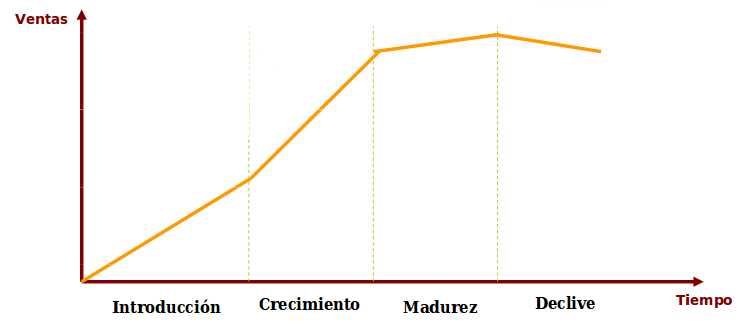
\includegraphics[width=0.8\textwidth]{2}
                \caption{Ciclo de vida del producto}
                \label{vida_p}
            \end{figure}

			El comportamiento de un producto (ventas y beneficios) varía desde el momento de su lanzamiento hasta que desaparece del mercado, como se ve en la \hyperref[vida_p]{Figura \ref*{vida_p}}. Hay cuatro etapas:

			\begin{description}
				\item[Etapa de introducción]: El nuevo producto empieza a distribuirse. Las empresas han de hacer un gran esfuerzo económico para hacer llegar el producto al público. Suele generar ventas muy bajas e incluso pérdidas, hasta que la sociedad comprenda su utilidad o ventaja respecto a otros productos.

				\item[Etapa de crecimiento]: El producto empieza a ser conocido en el mercado. Las ventas y beneficios suben rápidamente llegando a su nivel máximo. Aumenta la demanda hasta el punto de tener que ampliar los puntos de venta. Los competidores entran con sus propias marcas y este es el momento en el que la empresa debe usar estrategias de marketing para crear preferencia hacia sus productos.

				\item[Etapa de madurez]: Las ventas se estabilizan. Como los competidores ya están en el mercado, las estrategias de marketing suelen ser en vano e incluso generan pérdidas. Las acciones que se realizan ahora son bajar los precios y hacer menos publicidad y más acciones de promoción de ventas. Las cuotas de mercado de las distintas empresas se estabilizan.

				\item[Etapa de declive]: La aparición de nuevos productos sustitutivos que satisfacen las necesidades mejor que nuestros productos hacen que las ventas y los beneficios caigan. Esto hace que muchos competidores abandonen el producto y los precios se estabilicen. La empresa reduce las inversiones en el producto para sólo mantener a los consumidores fieles.
			\end{description}

	\section{\textcolor[rgb]{0.1,0.2,0.4}Decisiones de precio}

		El \textbf{precio} es la cantidad de dinero que un consumidor ha de desembolsar para disfrutar de un bien o servicio que le proporciona una utilidad. Dependiendo del tipo de producto o servicio del que estemos hablando, el precio recibe distintos nombres. Además, el precio tiene mucha importancia como instrumento de marketing. Los siguientes hechos lo justifican:
		\begin{description}
			\item[Efectividad a corto plazo]: Un cambio de precio puede hacerse en pocos días con efectos inmediatos sobre ventas y beneficios.

			\item[Efectividad como instrumento competitivo]: Una empresa puede revolucionar un sector con sólo utilizar el precio ya que el consumidor tiene una gran sensibilidad hacia éste.

			\item[Importantes repercusiones psicológicas sobre el consumidor]: Un precio alto puede hacer que el consumidor rechace comprarlo pero, si el precio es bajo, puede hacer también dudar al consumidor sobre su calidad.

			\item[En muchas decisiones de compra es la única información disponible]: cuando se desconoce el producto, la empresa fabricante o  su calidad el único indicador sobre la decisión de comprarlo es el precio.
		\end{description}

	\subsubsection{\textcolor[rgb]{0.1,0.2,0.4}Métodos de fijación de precios}

		\begin{description}
			\item[Métodos basados en los costes]: Estos métodos tienen una gran limitación: no tienen en cuenta aspectos como el nivel de competencia o diferenciación.
			\begin{enumerate}
				\item \textit{\textcolor[rgb]{0.1,0.2,0.4}{Coste más margen}}: consiste en que la empresa calcula el coste unitario de fabricación de un producto y le aplica un margen, para obtener el precio de venta al público.
				\item \textit{\textcolor[rgb]{0.1,0.2,0.4}{Margen en el precio}}: También tiene en cuenta los costes, pero el porcentaje de margen se aplica sobre el precio de venta.
				\item \textit{\textcolor[rgb]{0.1,0.2,0.4}{Precio objetivo}}: Aquí la empresa tiene en cuenta, además, el beneficio que quiere obtener. El precio de venta de cada unidad se obtiene añadiendo al coste total unitario, el beneficio por unidad que se quiere alcanzar.
			\end{enumerate}
			\item[Métodos basados en la competencia]: Se basan en el carácter competitivo de un mercado. Se tiene cuenta el coste ya que no se puede ofrecer un precio inferior a los costes.
			\begin{enumerate}
				\item \textit{\textcolor[rgb]{0.1,0.2,0.4}{Limitación o propuesta sellada}}: se da en mercados como la construcción o la contratación pública donde gana la empresa que, cumpliendo las condiciones preestablecidas por el cliente, ofrece el menor precio. Cuanto más bajo el precio más posibilidades de ser contratadas pero menor beneficio obtendrán.
				\item \textit{\textcolor[rgb]{0.1,0.2,0.4}{Precios similares a los competidores}}: se basan en el supuesto de que muchas empresas haciendo lo mismo no pueden estar equivocadas. Se comete el error de ignorar que la situación de nuestra empresa puede no ser la misma que la de los demás.
			\end{enumerate}
		\end{description}

		\subsubsection{\textcolor[rgb]{0.1,0.2,0.4}Estrategias de fijación de precios}

			Los métodos vistos sirven para la maximización a corto plazo, pero muchas veces las empresas están dispuestas a renunciar a un beneficio inmediato para obtener uno mayor en el futuro. Las estrategias son:
			\begin{description}
				\item[Productos nuevos]: 
				\begin{enumerate}
					\item \textit{\textcolor[rgb]{0.1,0.2,0.4}{Estrategia de penetración}}: Consiste en fijar precios bajos desde el lanzamiento de un producto para conseguir la mayor cuota de mercado posible. Es recomendable para productos que no son una auténtica novedad y estamos en un mercado sensible al precio, ya que con un precio bajo y poco margen, no resulta atractivo para los competidores potenciales.
					\item \textit{\textcolor[rgb]{0.1,0.2,0.4}{Estrategia de desnatado}}: Es el planteamiento contrario. La empresa fija un precio alto y mucha inversión en marketing para poder captar a aquellos clientes capaces de pagar los que sea por los productos, después, el precio irá bajando poco a poco para captar al resto de consumidores. Este planteamiento es recomendable para productos que suponen una novedad y son difícilmente imitables (para alejar a los competidores).
				\end{enumerate}
				\item[Precios para líneas de productos]: Hay que darse cuenta de que el precio de un producto afectará a la demanda del resto de productos de la línea y de otras líneas, por eso no podemos poner el precio producto a producto sin tener en cuenta el resto.
				\begin{enumerate}
					\item \textit{\textcolor[rgb]{0.1,0.2,0.4}{Líder de pérdidas}}: consiste en tener uno o dos productos de la línea a precios muy bajos para atraer a nuevos consumidores y ayuden a la venta de otros productos de mayor precio y margen. Es una técnica muy habitual entre los minoristas y por ejemplo en la informática, donde se vende una impresora muy barata pero obliga a la compra de tinta muy cara (\textbf{precio de productos cautivos}).
					\item \textit{\textcolor[rgb]{0.1,0.2,0.4}{Precio en dos partes}}: El precio se divide en una parte fija que da derecho al uso del servicio y otra variable en función del consumo. Habitual en telecomunicaciones.
					\item \textit{\textcolor[rgb]{0.1,0.2,0.4}{Precio único}}: Consiste en ofrecer todos los productos de una línea a un mismo precio. La lógica reside en que el consumidor a la hora de elegir olvida el precio (al ser común) y se fija en otros aspectos, facilitando la decisión de compra.
					\item \textit{\textcolor[rgb]{0.1,0.2,0.4}{Precio por paquete}}: Consiste en ofrecer un conjunto de productos a un precio inferior al que costarían si se compraran cada uno por separado. El consumidor no hubiera comprado todos los productos, pero el ahorro potencial le induce a ello.
				\end{enumerate}
				\item[Discriminación de precios]: Tiene lugar cuando la empresa vende el mismo producto a precios distintos porque ha sido capaz de encontrar segmentos de mercado dispuestos a pagar precios distintos:
				\begin{enumerate}
					\item \textit{\textcolor[rgb]{0.1,0.2,0.4}{Segmentos de consumidores}}: La empresa encuentra consumidores con distintas capacidades adquisitivas y adapta los precios a ellas.
					\item \textit{\textcolor[rgb]{0.1,0.2,0.4}{Criterios geográficos}}: La empresa fija precios distintos en regiones o países distintos.
					\item \textit{\textcolor[rgb]{0.1,0.2,0.4}{En función del tiempo}}.
				\end{enumerate}
				\item[Precios psicológicos]: basados en la percepción subjetiva del precio que tiene un consumidor en función de determinadas características que son manipulables, como por ejemplo:
				\begin{enumerate}
					\item \textit{\textcolor[rgb]{0.1,0.2,0.4}{Precios de prestigio}}: muchos consumidores asocian precio y calidad. Si el consumidor no tiene tiempo para medir otras variables, el precio es el único indicador, la empresa puede arriesgarse a poner un elevado precio a productos de calidad comparables a cualquier otro.
					\item \textit{\textcolor[rgb]{0.1,0.2,0.4}{Precio par o impar}}: los precios pares intentan hacer percibir el precio como inferior (en las ofertas se usa 19.9 frente a 20 para que parezca más barato), los precios pares se usan para facilitar el cobro y reducir las monedas fraccionarias.
					\item \textit{\textcolor[rgb]{0.1,0.2,0.4}{Precio acostumbrado}}: Muchos productos de precio bajo acaban teniendo un precio idéntico o similar que suele estar asociado a las monedas fraccionarias que hay en el mercado y ello lo hace muy difícil de modificar.
				\end{enumerate}
			\end{description}

	\section{\textcolor[rgb]{0.1,0.2,0.4}Decisiones de distribución}

		La función de distribución se encarga de poner al alcance físico del consumidor el producto en el momento, lugar y cantidad que necesita. Las distintas etapas por las que pasa el producto desde el fabricante al consumidor configuran el \textit{\textcolor[rgb]{0.1,0.2,0.4}{canal de distribución}}. El conjunto de personas que están entre el productor y el consumidor con los \textit{\textcolor[rgb]{0.1,0.2,0.4}{intermediarios}}. 

		\subsubsection{\textcolor[rgb]{0.1,0.2,0.4}Funciones de los intermediarios}

			Por cumplir estas funciones, el intermediario se queda con una parte del margen.

			\begin{enumerate}
				\item Reducen el número de transacciones (no sólo facilitan los intercambios, también los simplifican).
				\item Adecua la oferta a la demanda (de dos formas: porque compra grandes cantidades de productos y lo fracciona en más pequeñas y agrupa la producción de muchos pequeños fabricantes cuando cada uno ofrece cantidades muy pequeñas).
				\item Crea surtido (El distribuidor pone a disposición del consumidor un gran surtido de marcas sonde comparar y elegir).
				\item Almacena los productos, los transporta y los entrega.
				\item Financia el proceso (Los intermediarios proporcionan crédito tanto al fabricante como al consumidor).
				\item Asume riesgos (Cuando el intermediario adquiere un producto asume el riesgo de no poder venderlo, tener que bajar el precio por debajo del de compra, riesgo de robo, etc.)
			\end{enumerate}

		Las decisiones que adoptar un director de marketing en los referente a esta  herramienta son:
		\begin{enumerate}
			\item Determinar qué tipo de canal quiere para comercializar sus productos, establecer la longitud (decisión vertical) deseable de su canal. Las opciones por las que puede optar son:
			\begin{itemize} 
				\item \textit{\textcolor[rgb]{0.1,0.2,0.4}{canal ultra-corto o directo}} vendiendo sus productos directamente al consumidor (marketing directo). 
				\item \textit{\textcolor[rgb]{0.1,0.2,0.4}{canal corto}}, donde existe un único intermediario entre el fabricante y el consumidor, que suele ser, un minorista\footnote{Llamamos minorista al intermediario que vende al consumidor y mayorista al intermediario que vende a otros intermediarios}.
				\item \textit{\textcolor[rgb]{0.1,0.2,0.4}{canal largo}},  donde existen dos intermediarios, normalmente un mayorista y un minorista. El mayorista adquiere productos de distintos fabricantes y los envía a minoristas, a veces, cuando los minoristas tienen grandes capacidades de compra, se convierten en mayoristas.
			\end{itemize}
			\item Determinar el número y el tipo de minoristas que quiere que ofrezcan sus productos al consumidor (decisión vertical):
			\begin{itemize}
				\item \textit{\textcolor[rgb]{0.1,0.2,0.4}{Distribución exclusiva}}: El fabricante limita al máximo el número de minoristas, concediéndoles a éstos la exclusividad de venta de su producto a un área geográfica determinada y con la condición de que no vendan productos de otros fabricantes. Es habitual cuando son productos que exigen un gran esfuerzo de venta o van acompañados de servicios de asistencia técnica o reparación. Al concederle la exclusiva, el minorista puede conocer a fondo el producto y llevar a cabo un mayor esfuerzo de venta.
				\item \textit{\textcolor[rgb]{0.1,0.2,0.4}{Distribución selectiva}}: El número de minoristas en una zona es reducido pero no hay un único distribuidor. Al permitirse más de un minorista en la misma zona se le permite vender productos de otros fabricantes aunque en volúmenes mínimos de venta.
				\item \textit{\textcolor[rgb]{0.1,0.2,0.4}{Distribución intensiva}}: El fabricante recurre al máximo número posible de puntos de venta en una zona determinada, suele darse en productos de compra frecuente como la alimentación y va asociada a canales de distribución largos.
			\end{itemize}
		\end{enumerate}

		Por último, hay dos tipos de estrategias de distribución:
		\begin{description}
			\item[Push]: Consiste en incentivar al mayorista y al minorista a que compren nuestros productos con grandes descuentos por volumen y buenas condiciones de financiación. Una vez acumulado nuestro producto, se verá obligado a darle salida \textit{\textcolor[rgb]{0.1,0.2,0.4}{empujando}} el producto por el canal.
			\item[Pull]: La empresa hace grandes esfuerzos de comunicación con el consumidor final para que se interese por nuestro producto y lo pida a un minorista, el consumidor \textit{\textcolor[rgb]{0.1,0.2,0.4}{tira}} del producto por el canal.
		\end{description}

	\section{\textcolor[rgb]{0.1,0.2,0.4}Decisiones de comunicación}

		La empresa debe \textit{\textcolor[rgb]{0.1,0.2,0.4}{comunicar}} al mercado la existencia de su producto, sus características, qué lo hace distinto de los demás, a qué precios lo puede adquirir y dónde. Para ello dispone de las siguientes herramientas:
		\begin{description}
			\item[Publicidad]: en la publicidad la empresa transmite a través de un medio de comunicación de masas, información comercial relevante para el consumidor con el fin de estimular la demanda de su producto o servicio. Esta comunicación es unilateral, impersonal (se dirige a un público anónimo), y masiva. Con la publicidad la empresa busca:
			\begin{enumerate}
				\item Informar (hacer que el mercado sepa de la existencia de un nuevo producto e informar de sus características)
				\item Persuadir (hacer que el consumidor actúe de una determinada manera)
				\item Recordar (Mantener los niveles de recuerdo de marcas que llevan mucho tiempo en el mercado)
			\end{enumerate}
			Las empresas cuentan con la ayuda de \textit{\textcolor[rgb]{0.1,0.2,0.4}{agencias de publicidad}} para diseñar su publicidad. Éstas lo diseñan, lo producen, eligen los medios más adecuados para el tipo de anuncio realizado y los soportes. También deciden la programación de la campaña.
			\item[Promoción de ventas]: Pueden ser descuentos en precio, regalo de producto gratuito, regalo de producto diferente, degustaciones, sorteos, concursos... No es publicidad pero informa igualmente de ventajas del producto e incita a comprarlo.
			\item[Relaciones públicas]: Su objetivo es que la empresa mantenga una relación de confianza y entendimiento con la administración pública, sus propios trabajadores, accionistas...  Para ello el director de marketing dispone de diferentes instrumentos como la \textit{\textcolor[rgb]{0.1,0.2,0.4}{publicity}} o los \textit{\textcolor[rgb]{0.1,0.2,0.4}{patrocinios}}. Y para dirigirnos a accionistas, las \textit{\textcolor[rgb]{0.1,0.2,0.4}{memorias anuales}}, \textit{\textcolor[rgb]{0.1,0.2,0.4}{publicaciones de empresa}}, etc.
			\item[Marketing directo]: Hace referencia a acciones de comunicación entre el fabricante y el consumidor en las que este último puede demostrar una respuesta medible.
			\item[Venta personal]: La comunicación entre el vendedor y el cliente es interpersonal (es de doble sentido, el vendedor expone sus argumentos pero el cliente también). Es personal, se dirige a una persona concreta. Sin embargo, no hay que ignorar que la vena personal hace uso intensivo de un activo caro: el personal. Por lo que sólo se usa cuando la empresa ha optado por un canal de distribución largo.
			\item[Comunicación Integrada de Marketing (CIM)]: Las herramientas presentadas anteriormente se pueden combinar entre sí.
		\end{description}

\end{document}
\hyperref[empresa_abierta_regulada]{Figura \ref*{empresa_abierta_regulada}}
\textcolor[rgb]{0.1,0.2,0.4}
      \[\begin{xy}
            ,(0,0)*+=[o]=<3cm>[F]\txt<3cm>{Contexto de la estrategia de empresa, estructura y rivalidad en\\países}
            ,(0,60)*+=[o]=<3cm>[F]\txt<3cm>{Industrias de éxito\\{\tiny Industrias de soporte e industrias relacionadas}}
            ,(-60,30)*+=[o]=<3cm>[F]\txt<3cm>{Condiciones de los factores productivos específicos\\{\tiny Ventaja nacional}}
            ,(60,30)*+=[o]=<3cm>[F]\txt<3cm>{Condiciones de demanda nacional\\{\tiny Ventaja organizacional}}
            \ar@{<->} (0,15);(0,45)
            \ar@{<->} (-45,30-);(45,30)
            \ar@{<->} (0,45);(45,30)
            \ar@{<->} (45,30);(0,15)
            \ar@{<->} (0,15);(-45,30)
            \ar@{<->} (-45,30);(0,45)
      \end{xy}\]

 \begin{figure}
                  \centering
                  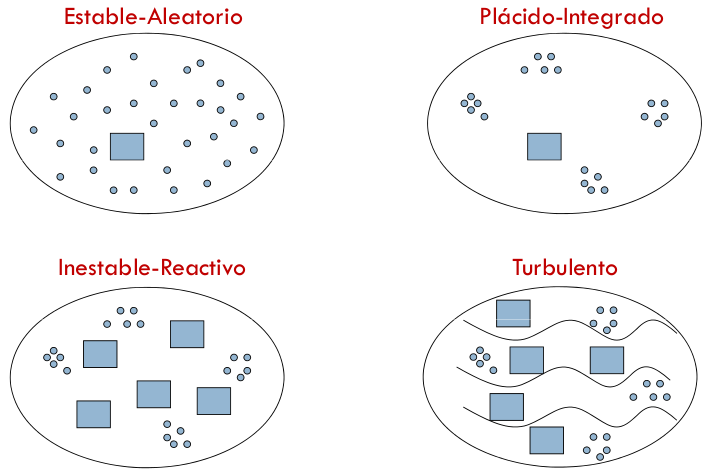
\includegraphics[width=0.8\textwidth]{1}
                  \caption{Tipos de entorno}
                  \label{tipos_entorno}
            \end{figure}